\section{Winter Recce, 29-30th Dec 2009}

The trip started, as all good things do, with a 5AM alpine start; we caught the first train out of \passage[town]{Most Na Soci} and through the Julian alps to \passage[town]{Bohinjska Bistrica}, then a bus to \passage{Hotel Zlatorog} near \passage[river]{Savica} (the possible Black Sea resurgence for the \passage{Migovec} systems). With ice axe and crampons a quick 1.2km of ascent saw us up on our beloved plateau, with \passage[mountain]{Tolminski Kuk} brooding in the cloud layer. Based at \passage{Dom na Komni}, we spent the next day in poor visibility logging 5 new blow holes and having a look at the N1-3 entrances.

\name{Jarvist Frost}


\begin{pagefigure}
\checkoddpage \ifoddpage \forcerectofloat \else \forceversofloat \fi
\frame{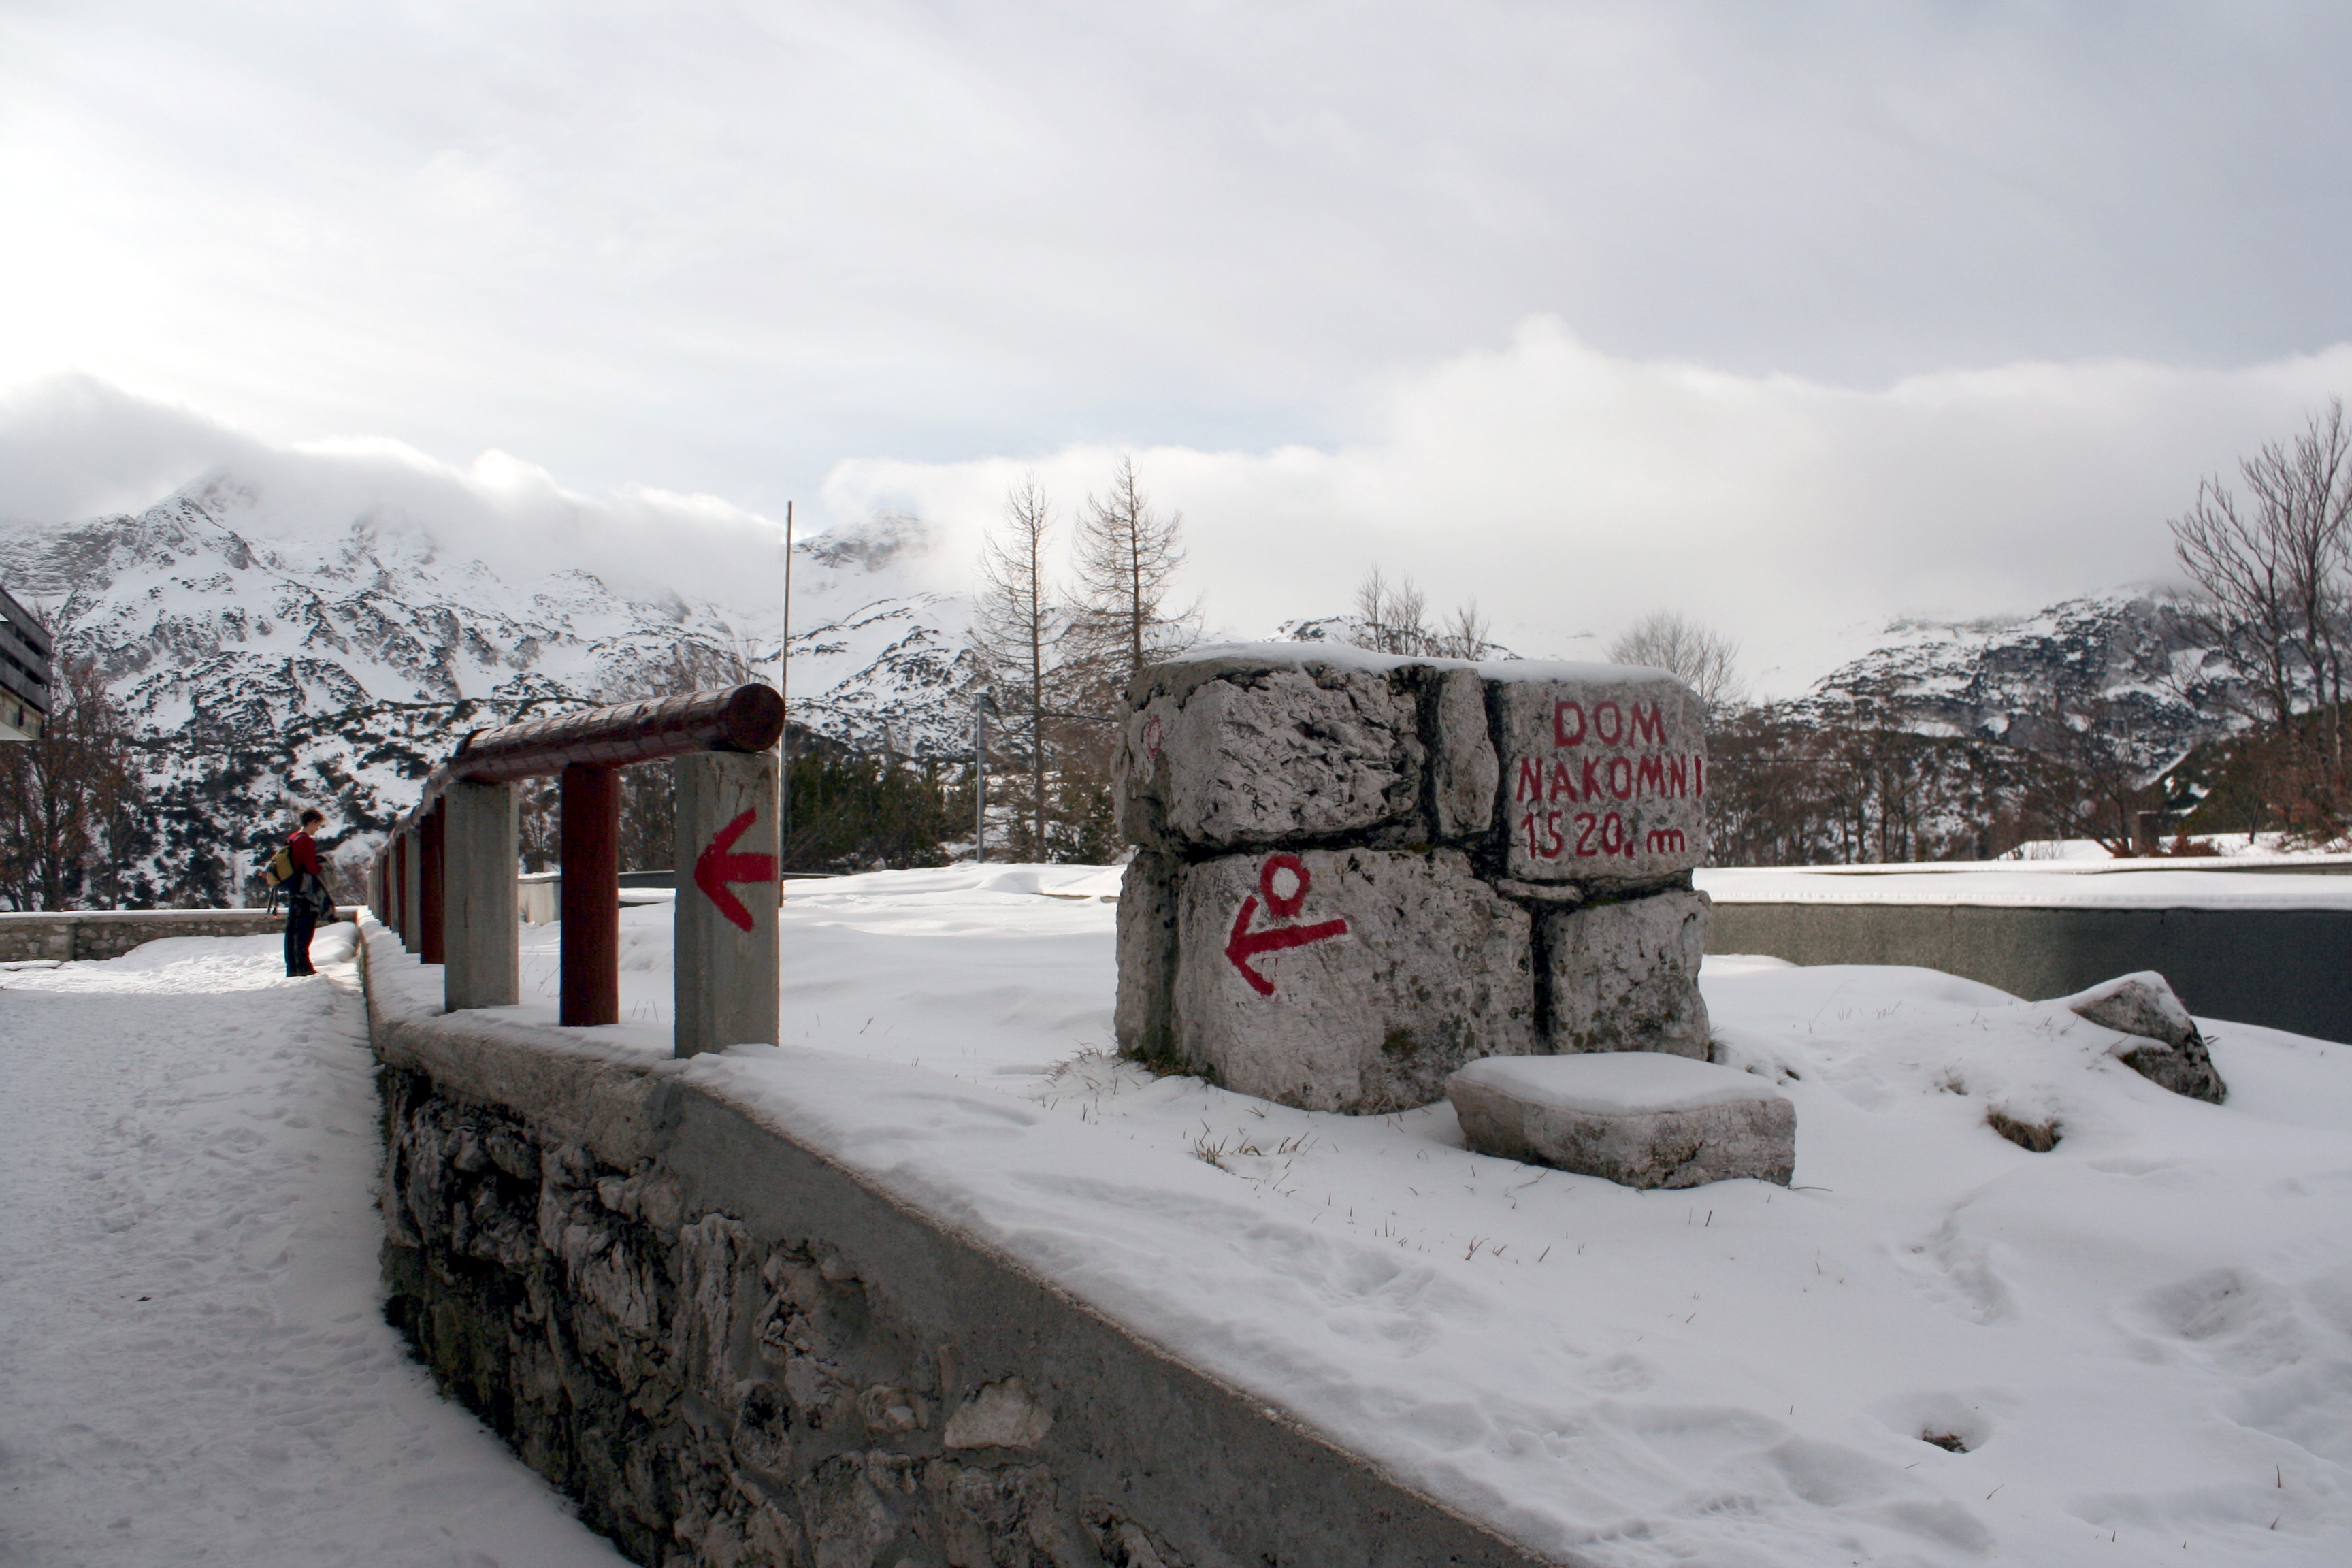
\includegraphics[width=\linewidth]{2009/winter_recce/2009-12-30 - Area N Winter Recce - Jana Carga - Canon 350d - IMG_7253-studying map and cloudy peaks at dom na komni 1520m--orig.jpg}}
\caption{Jarvist outside the refuge of \passage{Dom na Komni}, which lies 1520 m above sea level. The refuge is located to the north of \passage[mountain]{Migovec} and \passage[mountain]{Kuk}. \pic{Jana Čarga}} \label{Dom na Komni in snow}
\end{pagefigure}




\begin{pagefigure}
      \checkoddpage \ifoddpage \forcerectofloat \else \forceversofloat \fi
    \centering
    \begin{subfigure}{0.49\textwidth}
        \frame{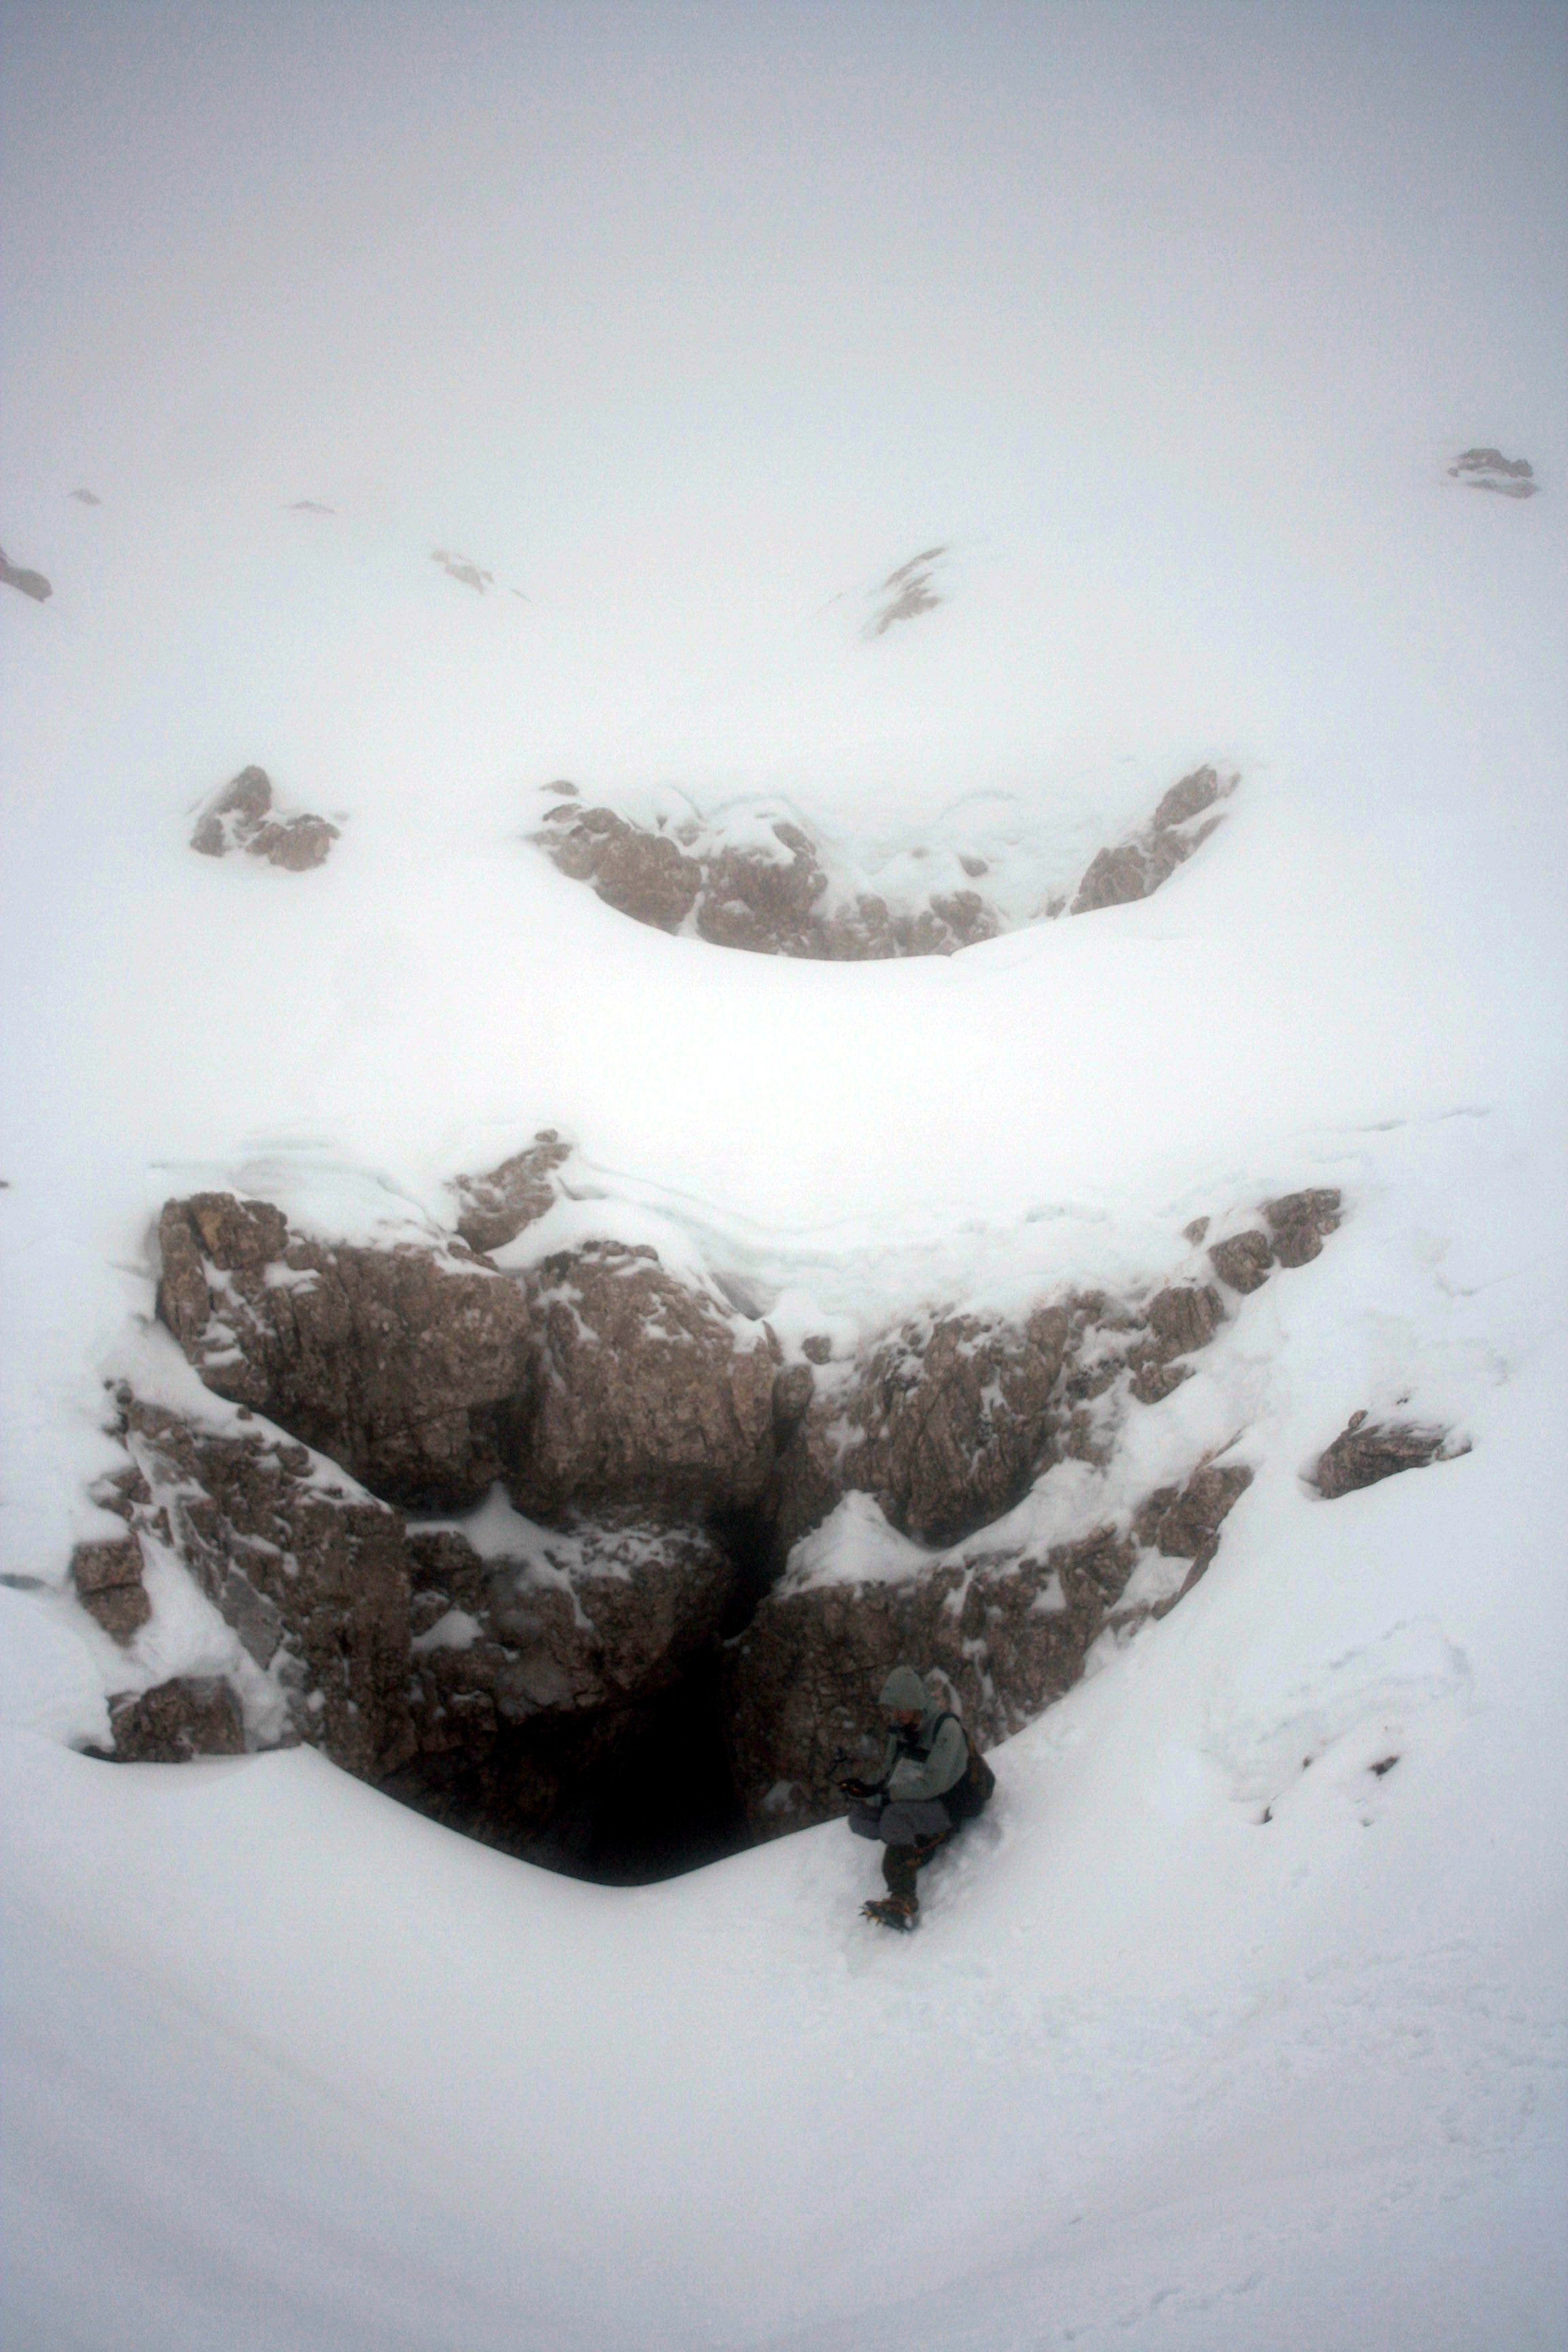
\includegraphics[width=\linewidth]{2009/winter_recce/2009-12-30 - Area N Winter Recce - Jana Carga - Canon 350d - IMG_7332-N1--orig.jpg}} 
        \caption{} \label{N1 1}
    \end{subfigure}
\hfill
    \begin{subfigure}{0.49\textwidth}
    \centering
        \frame{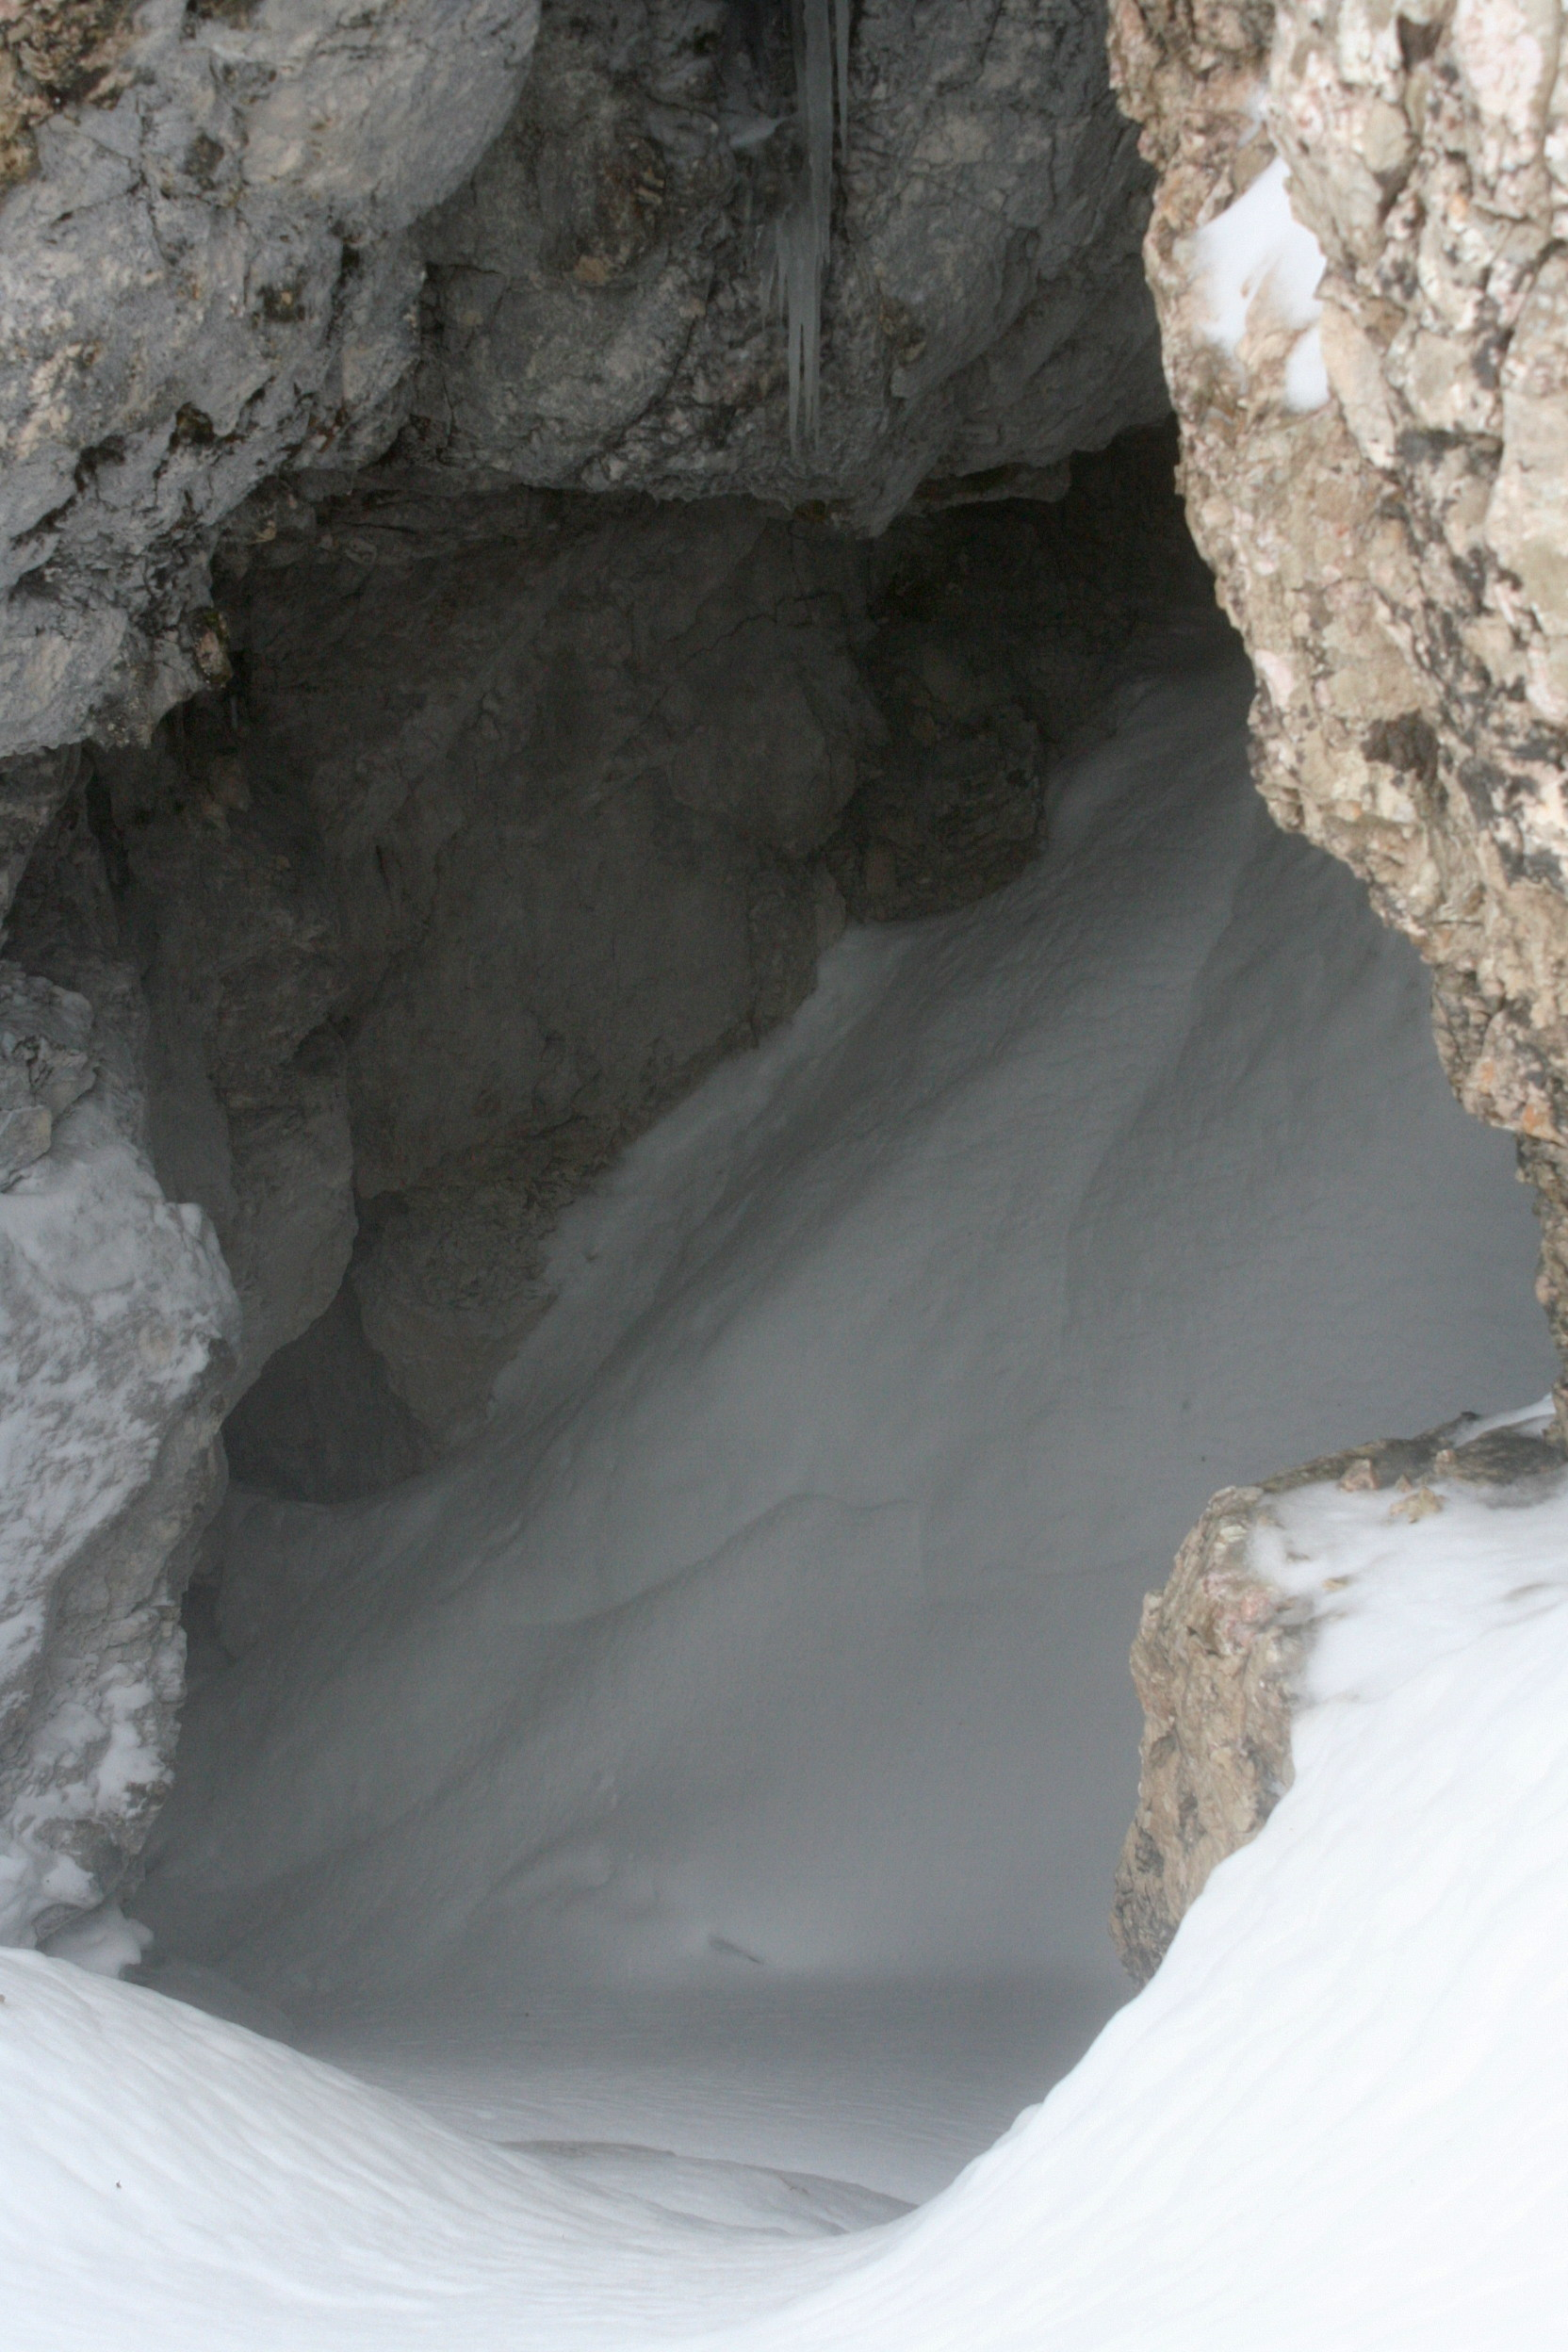
\includegraphics[width=\linewidth]{2009/winter_recce/2009-12-30 - Area N Winter Recce - Jana Carga - Canon 350d - IMG_7329-N1--orig.jpg}} 
        \caption{} \label{N1 2}
\end{subfigure}
\vfill
\begin{subfigure}{0.49\textwidth}
    \centering
        \frame{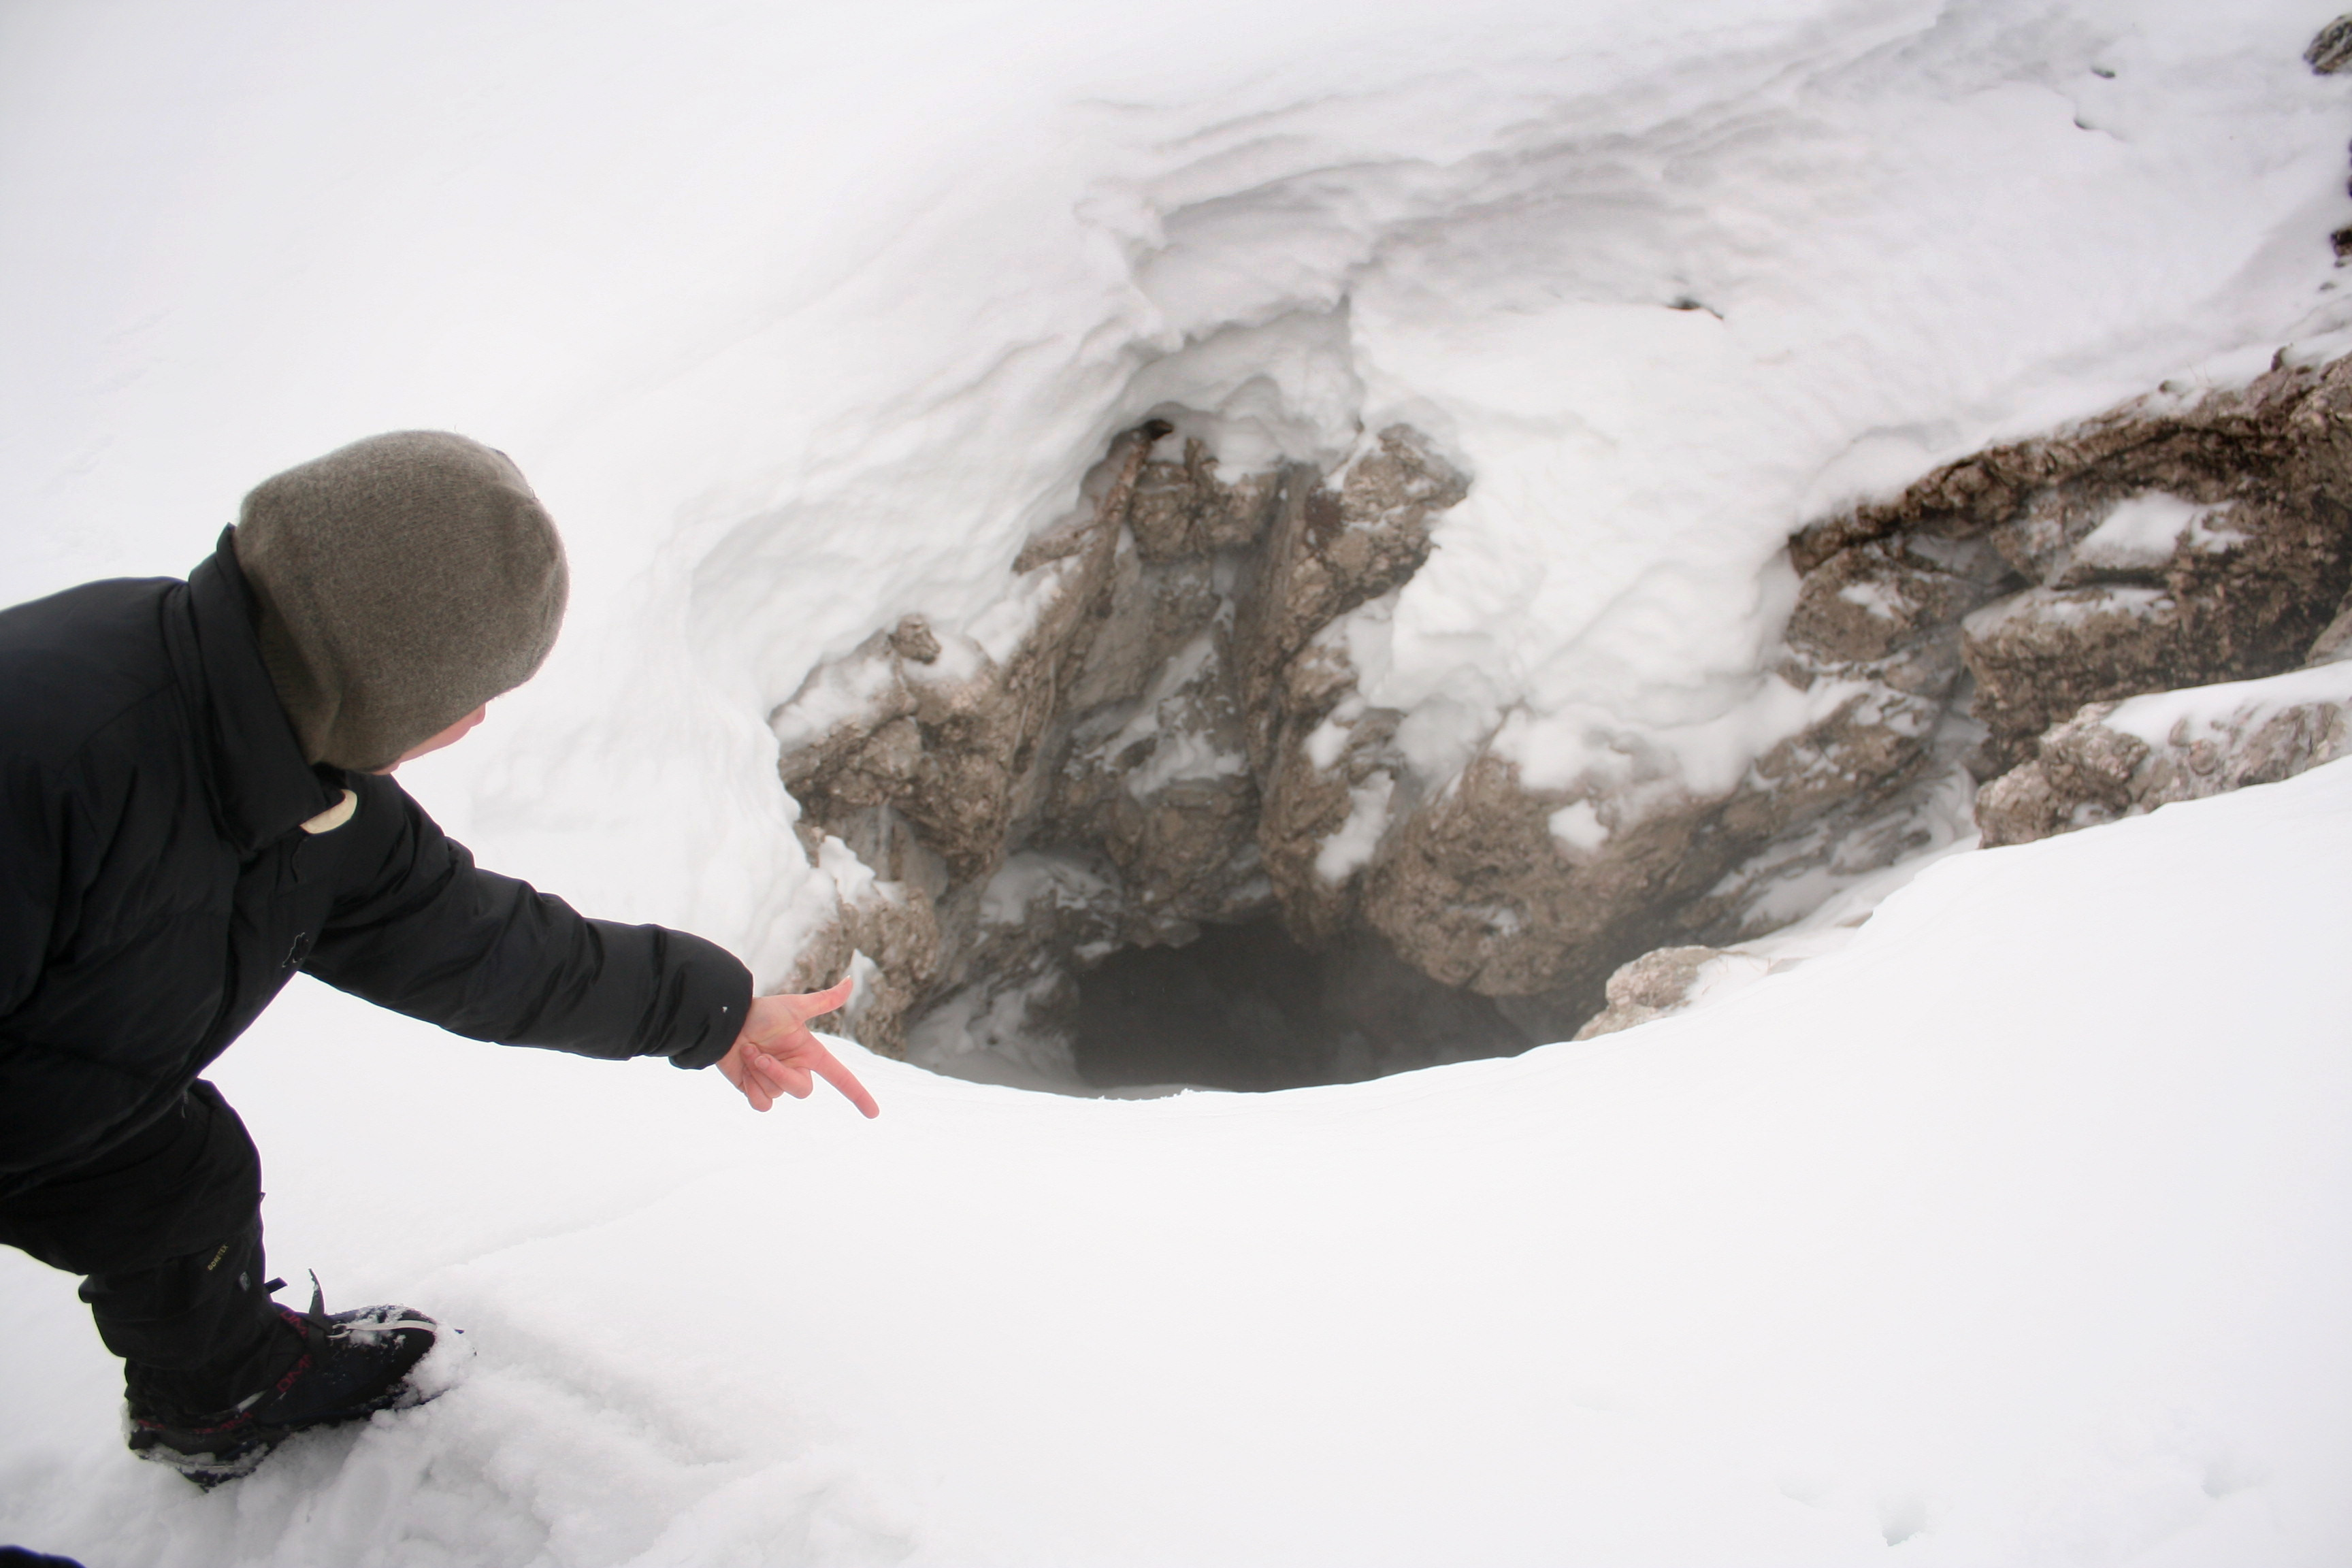
\includegraphics[width=\linewidth]{2009/winter_recce/2009-12-30 - Area N Winter Recce - Jana Carga - Canon 350d - IMG_7323-N2--orig.jpg}} 
        \caption{} \label{N2 1}
\end{subfigure}
\hfill
\begin{subfigure}{0.49\textwidth}
    \centering
        \frame{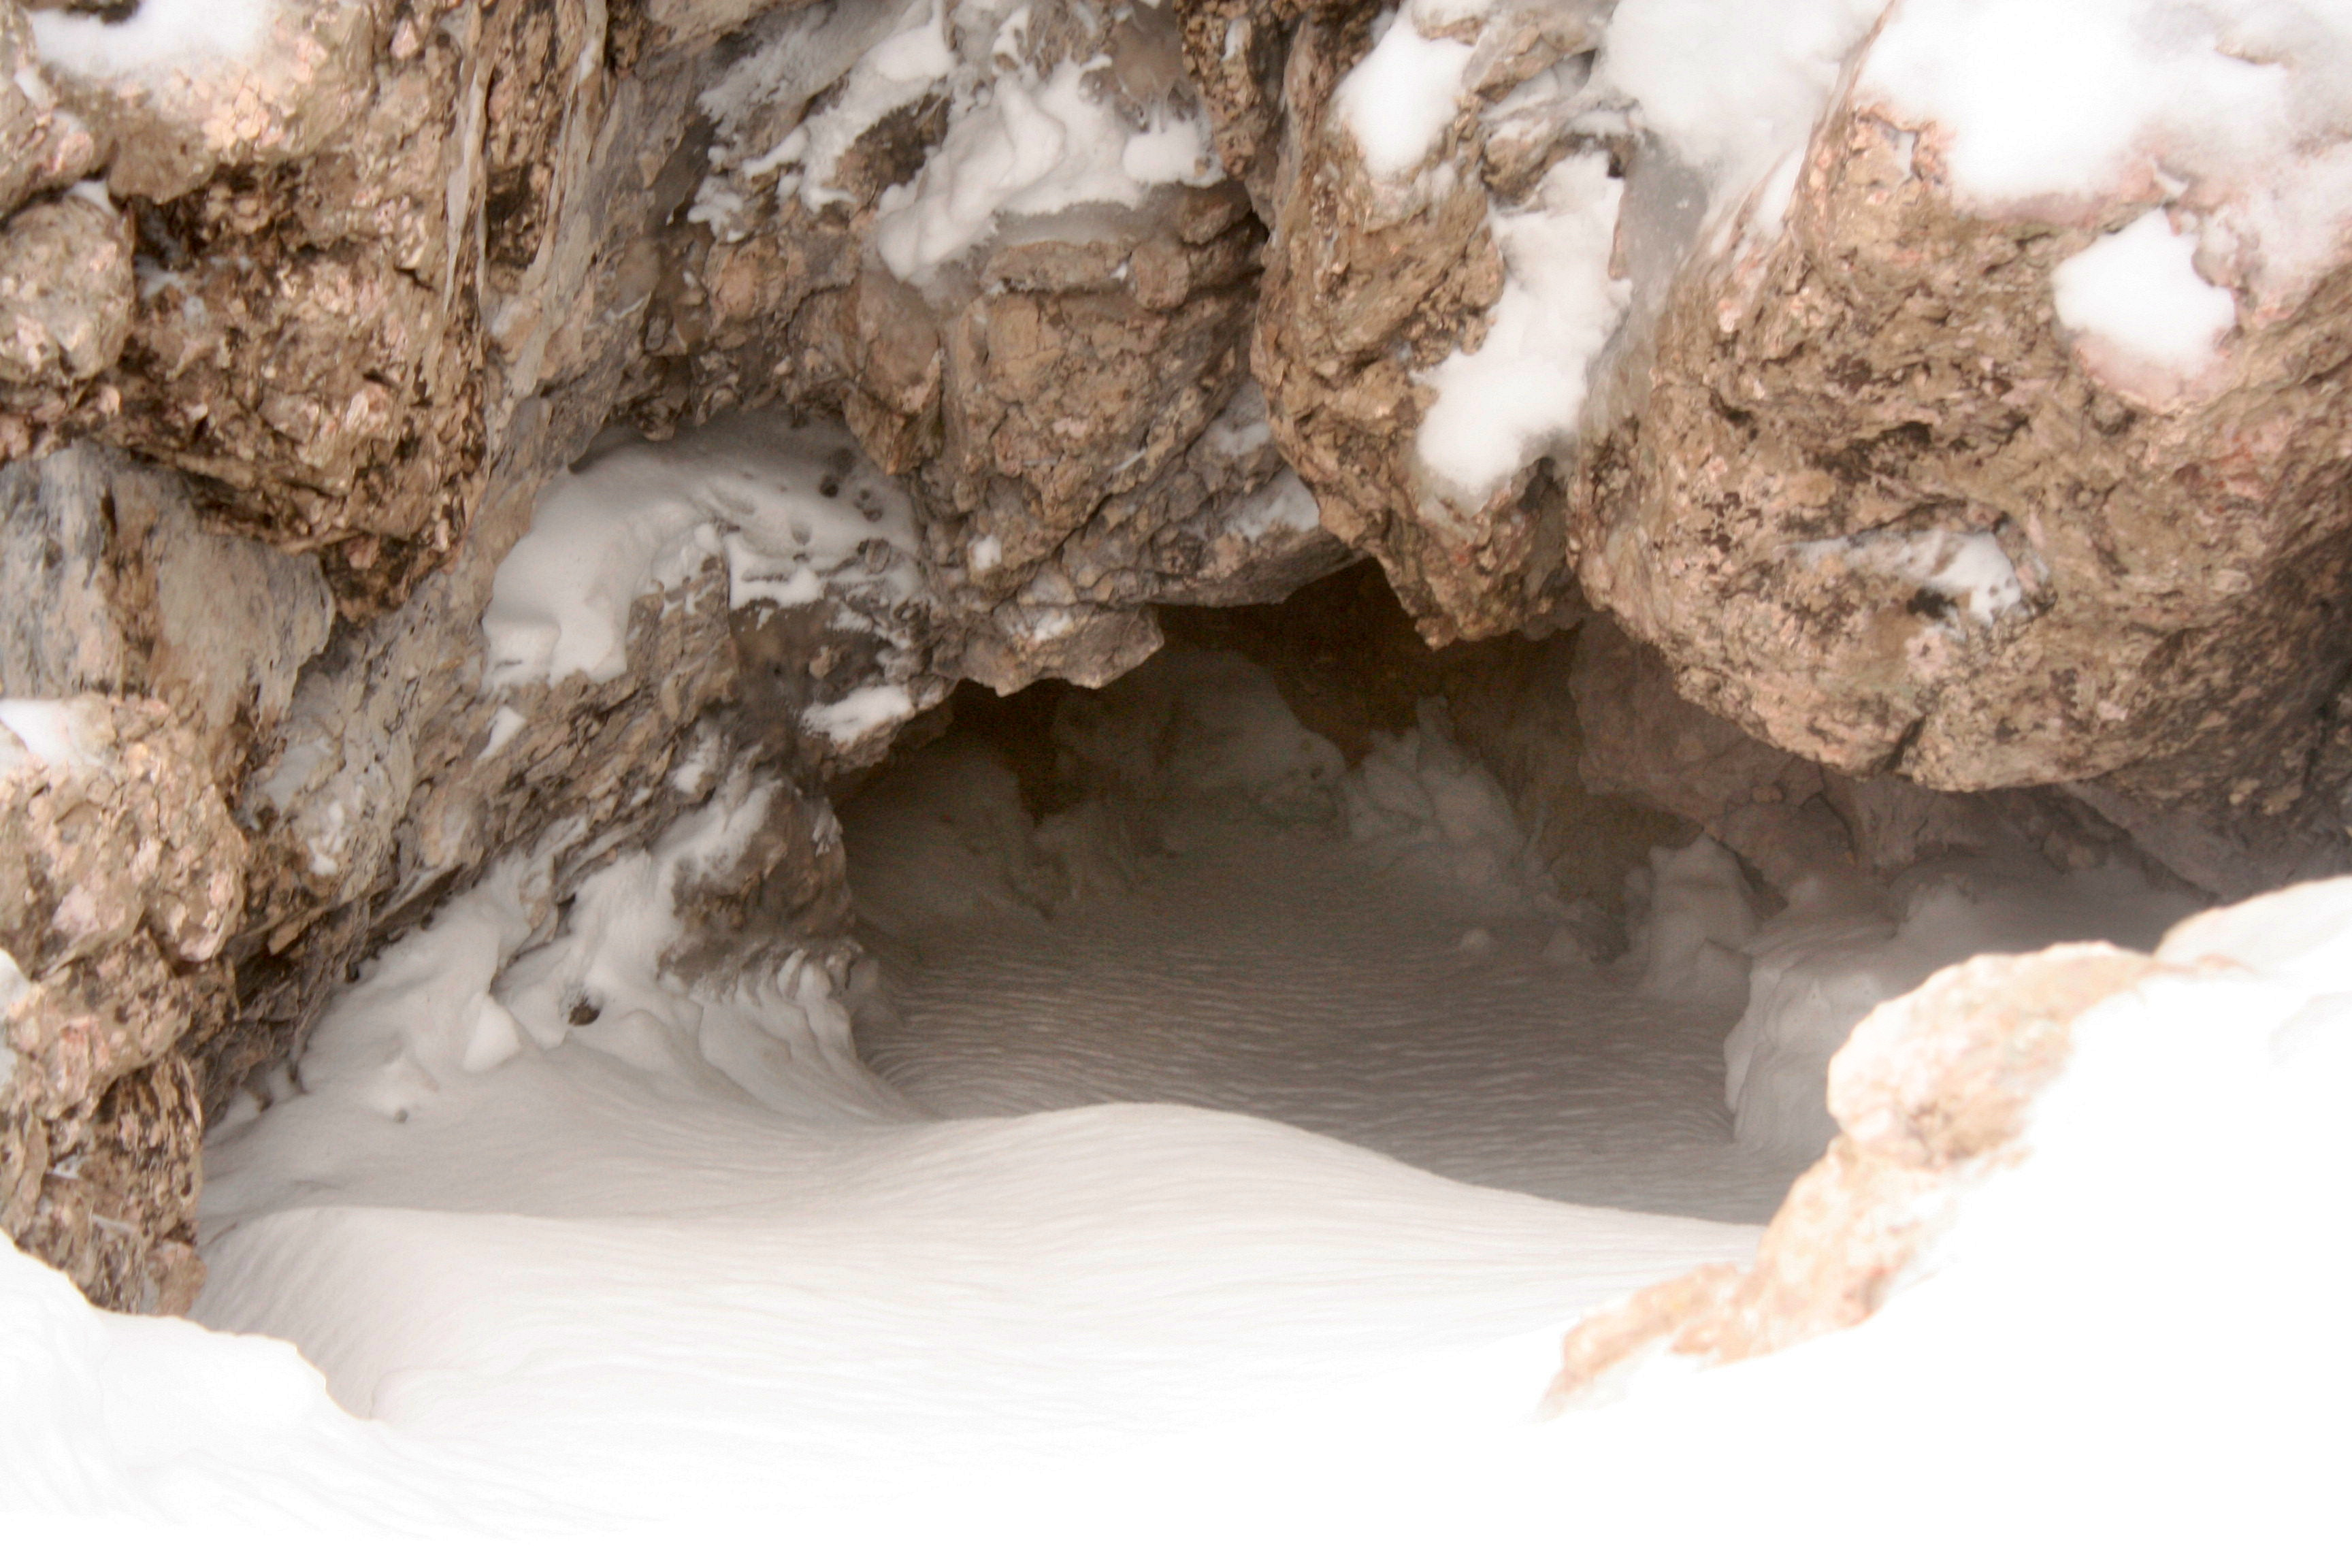
\includegraphics[width=\linewidth]{2009/winter_recce/2009-12-30 - Area N Winter Recce - Jana Carga - Canon 350d - IMG_7322-looking into N2--orig.jpg}}
        \caption{} \label{N2 2}
    \end{subfigure}
 \caption{\protect\passage{N1} and \protect\passage{N2}. \textit{(a)} The entrance of \protect\passage{N1}. \textit{(b)} Looking into \protect\passage{N1}. \textit{(c)} The entrance of \protect\passage{N2}. \textit{(d)} Looking into \protect\passage{N2}. \pic{Jana Čarga / Jarvist Frost} }
\end{pagefigure}


















\begin{pagefigure}
      \checkoddpage \ifoddpage \forcerectofloat \else \forceversofloat \fi
    \centering
    \begin{subfigure}{0.49\textwidth}
        \frame{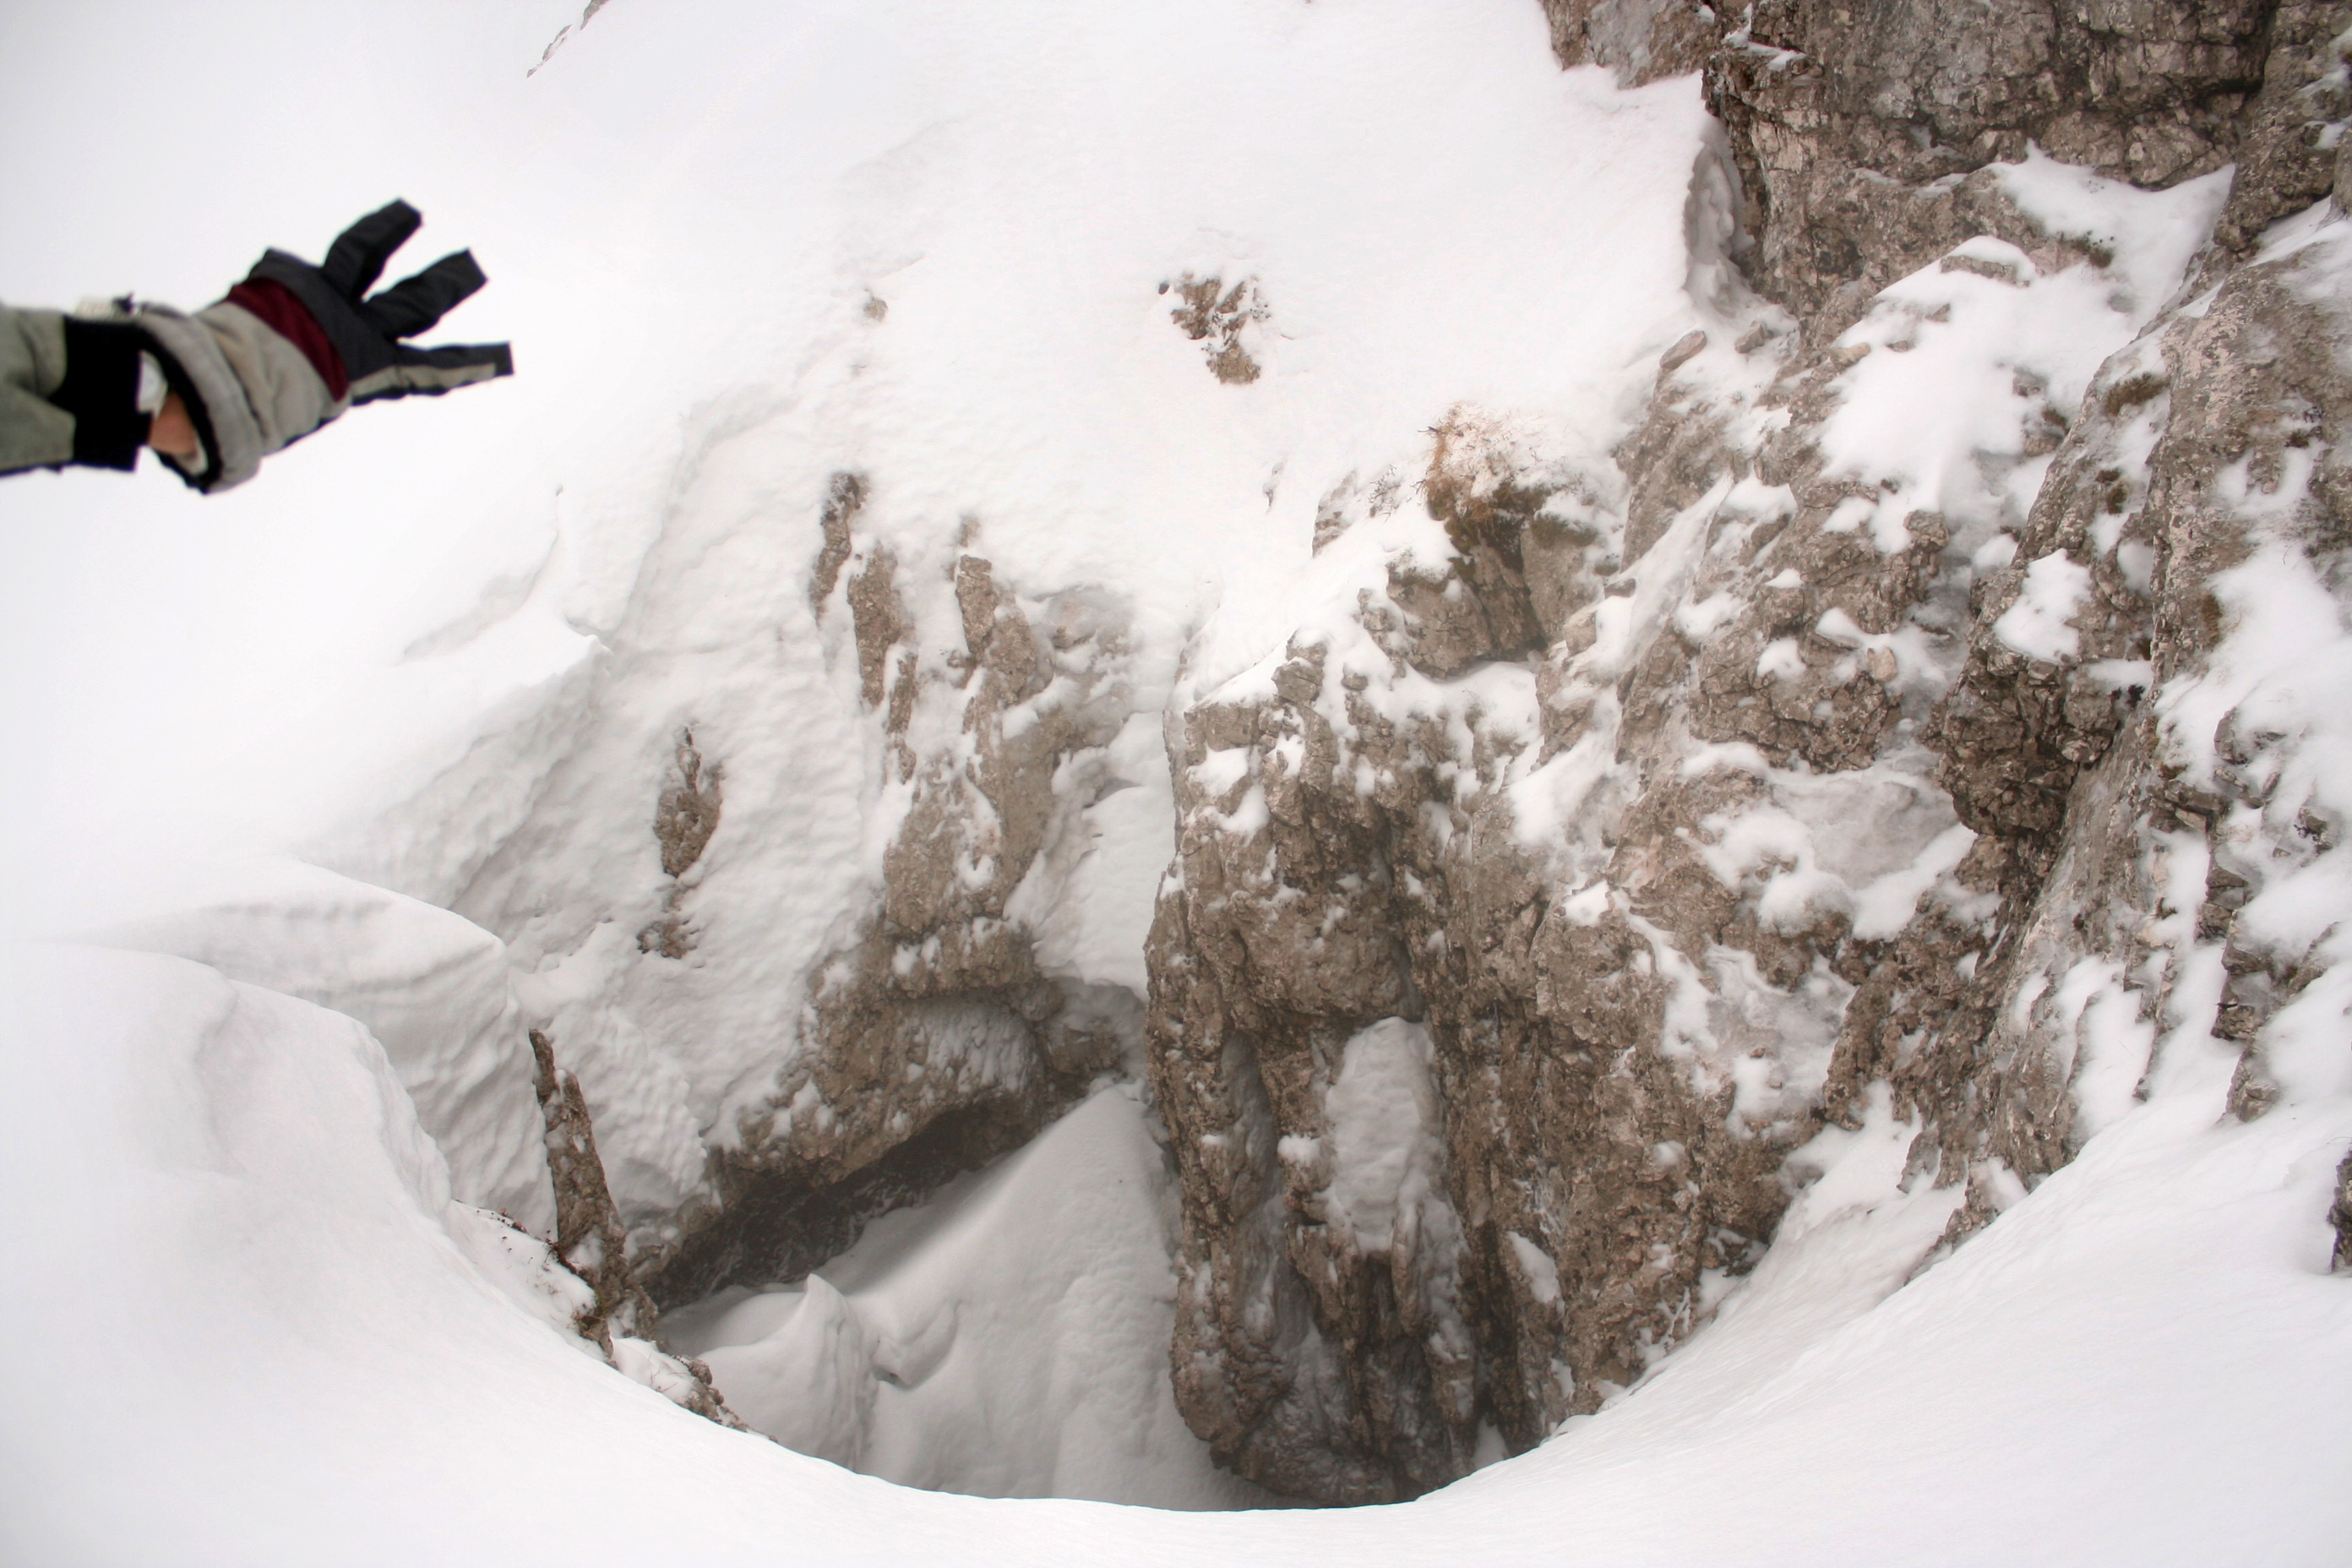
\includegraphics[width=\linewidth]{2009/winter_recce/2009-12-30 - Area N Winter Recce - Jana Carga - Canon 350d - IMG_7325-N3--orig.jpg}} 
        \caption{} \label{N3}
    \end{subfigure}
\hfill
    \begin{subfigure}{0.49\textwidth}
    \centering
        \frame{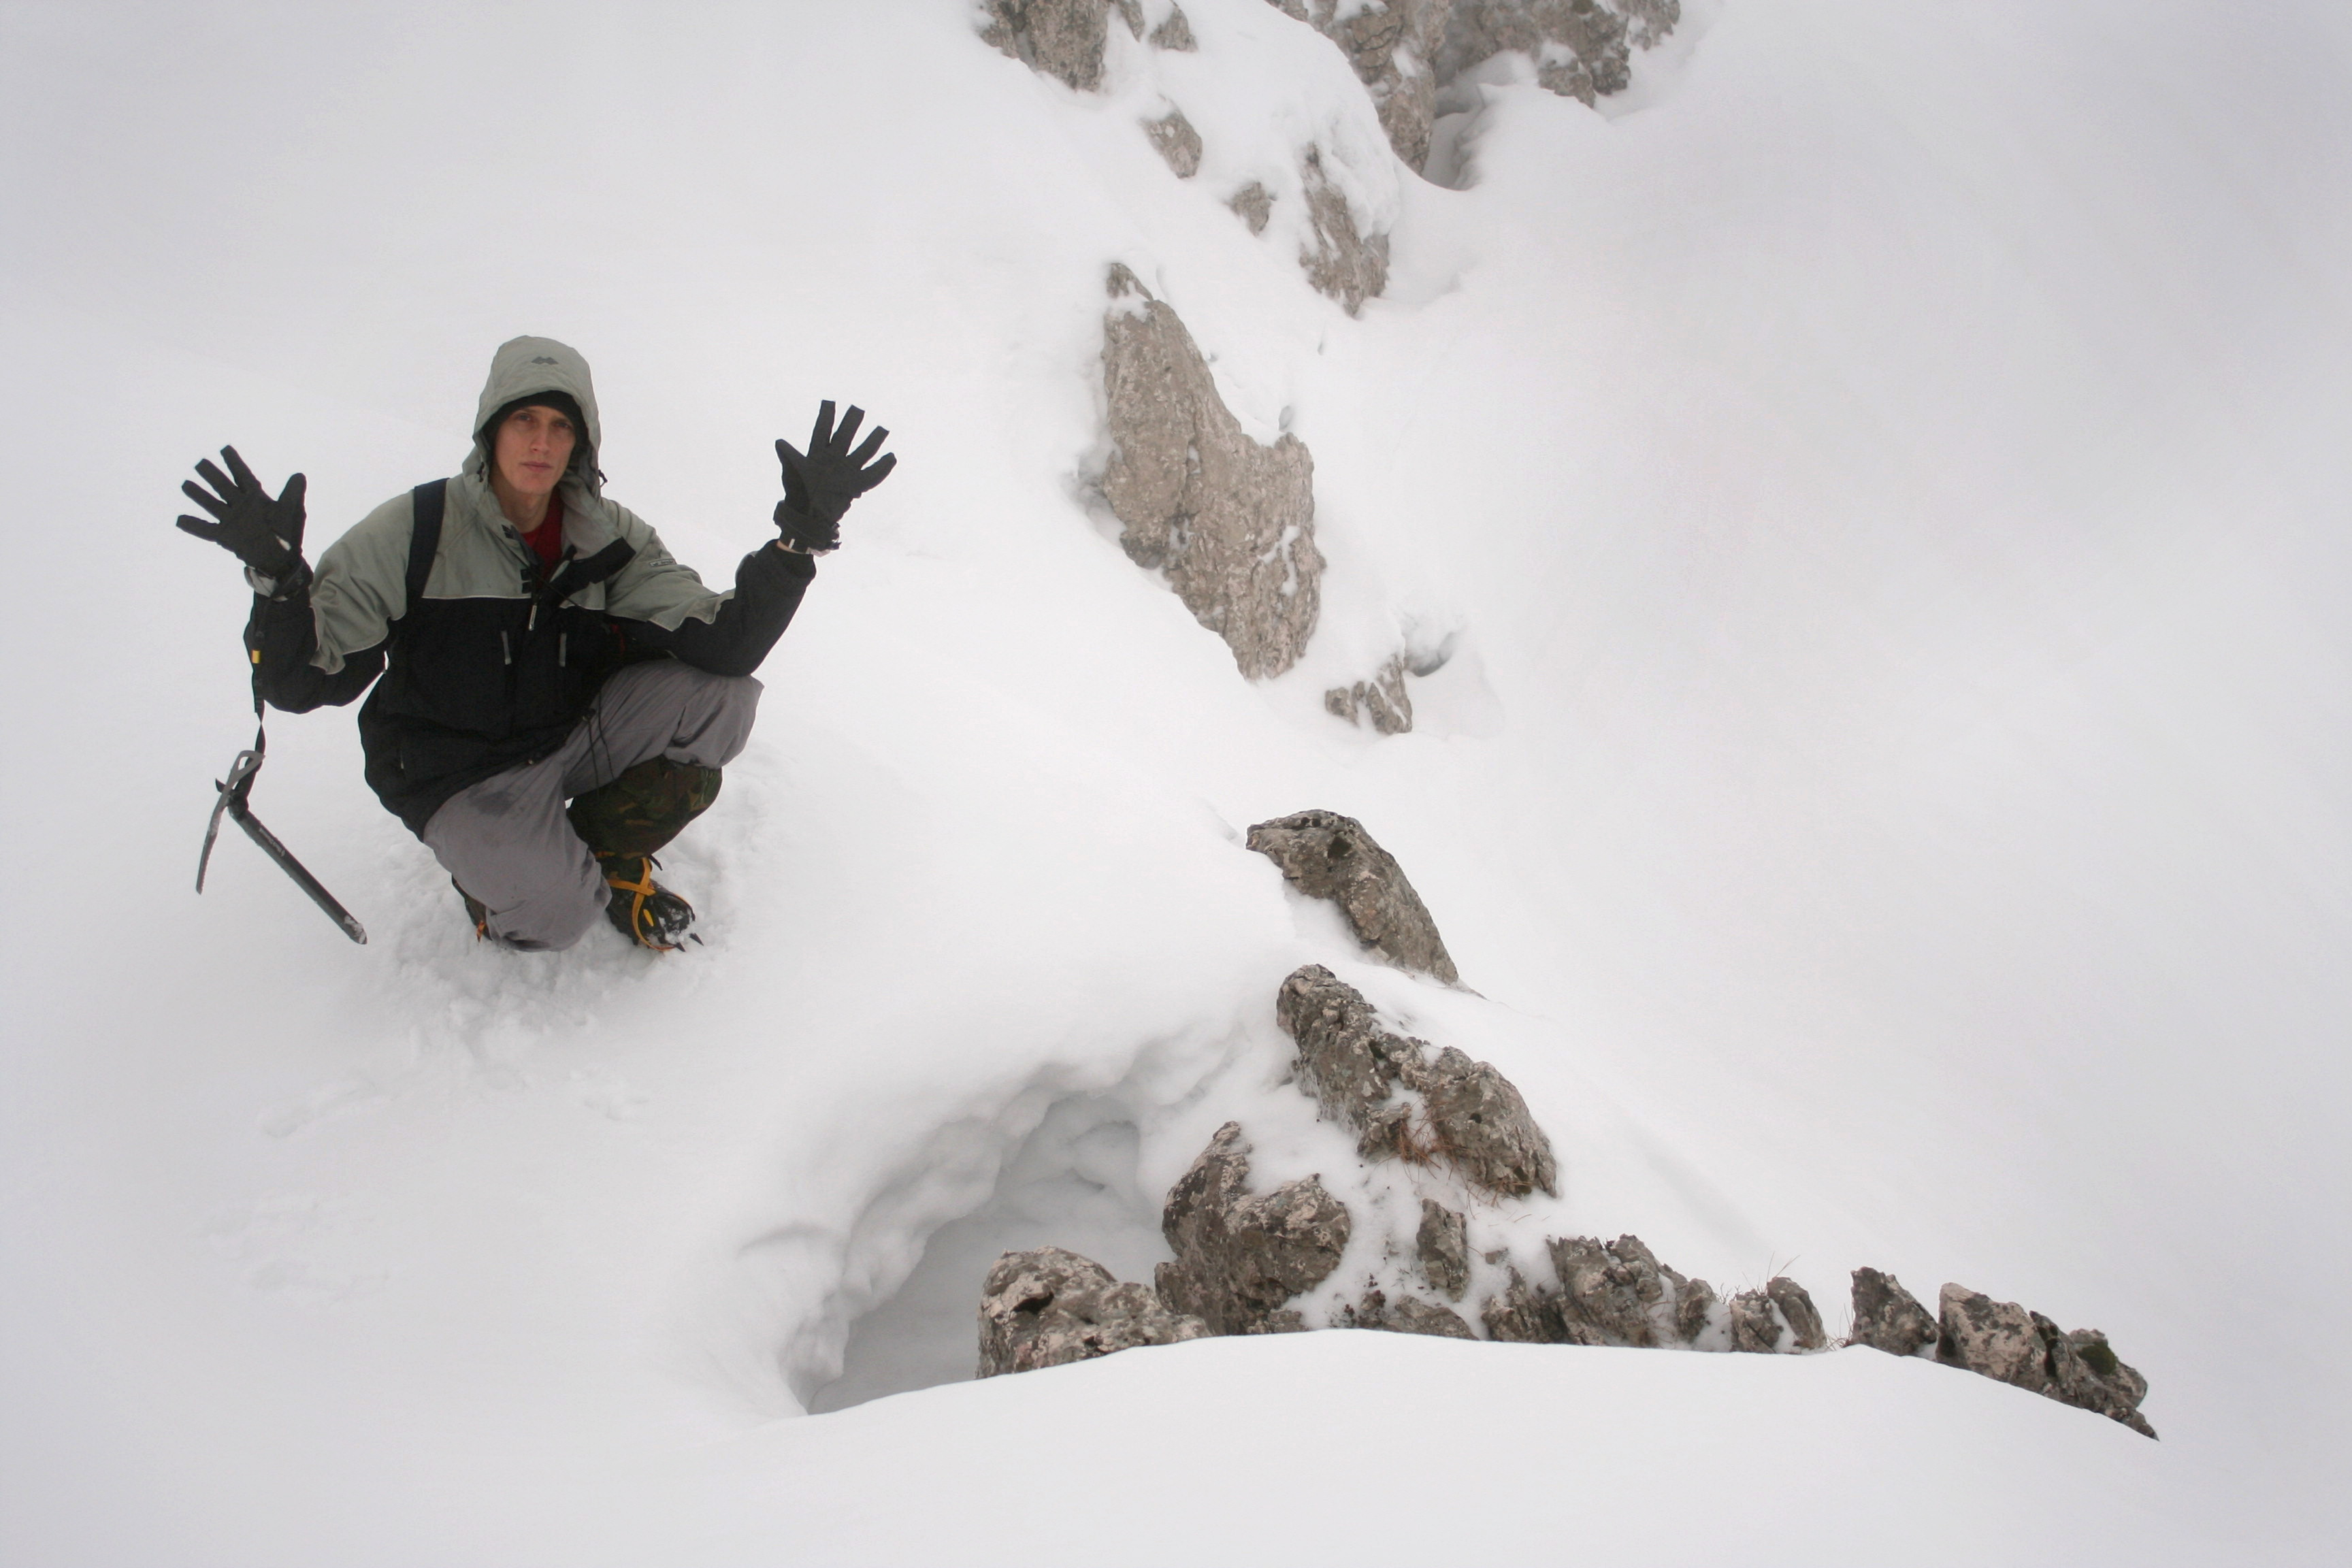
\includegraphics[width=\linewidth]{2009/winter_recce/2009-12-30 - Area N Winter Recce - Jana Carga - Canon 350d - IMG_7318-jarv next to N10 with N3 in background across valley--orig.jpg}} 
        \caption{} \label{N10}
\end{subfigure}
\vfill
\begin{subfigure}{0.49\textwidth}
    \centering
        \frame{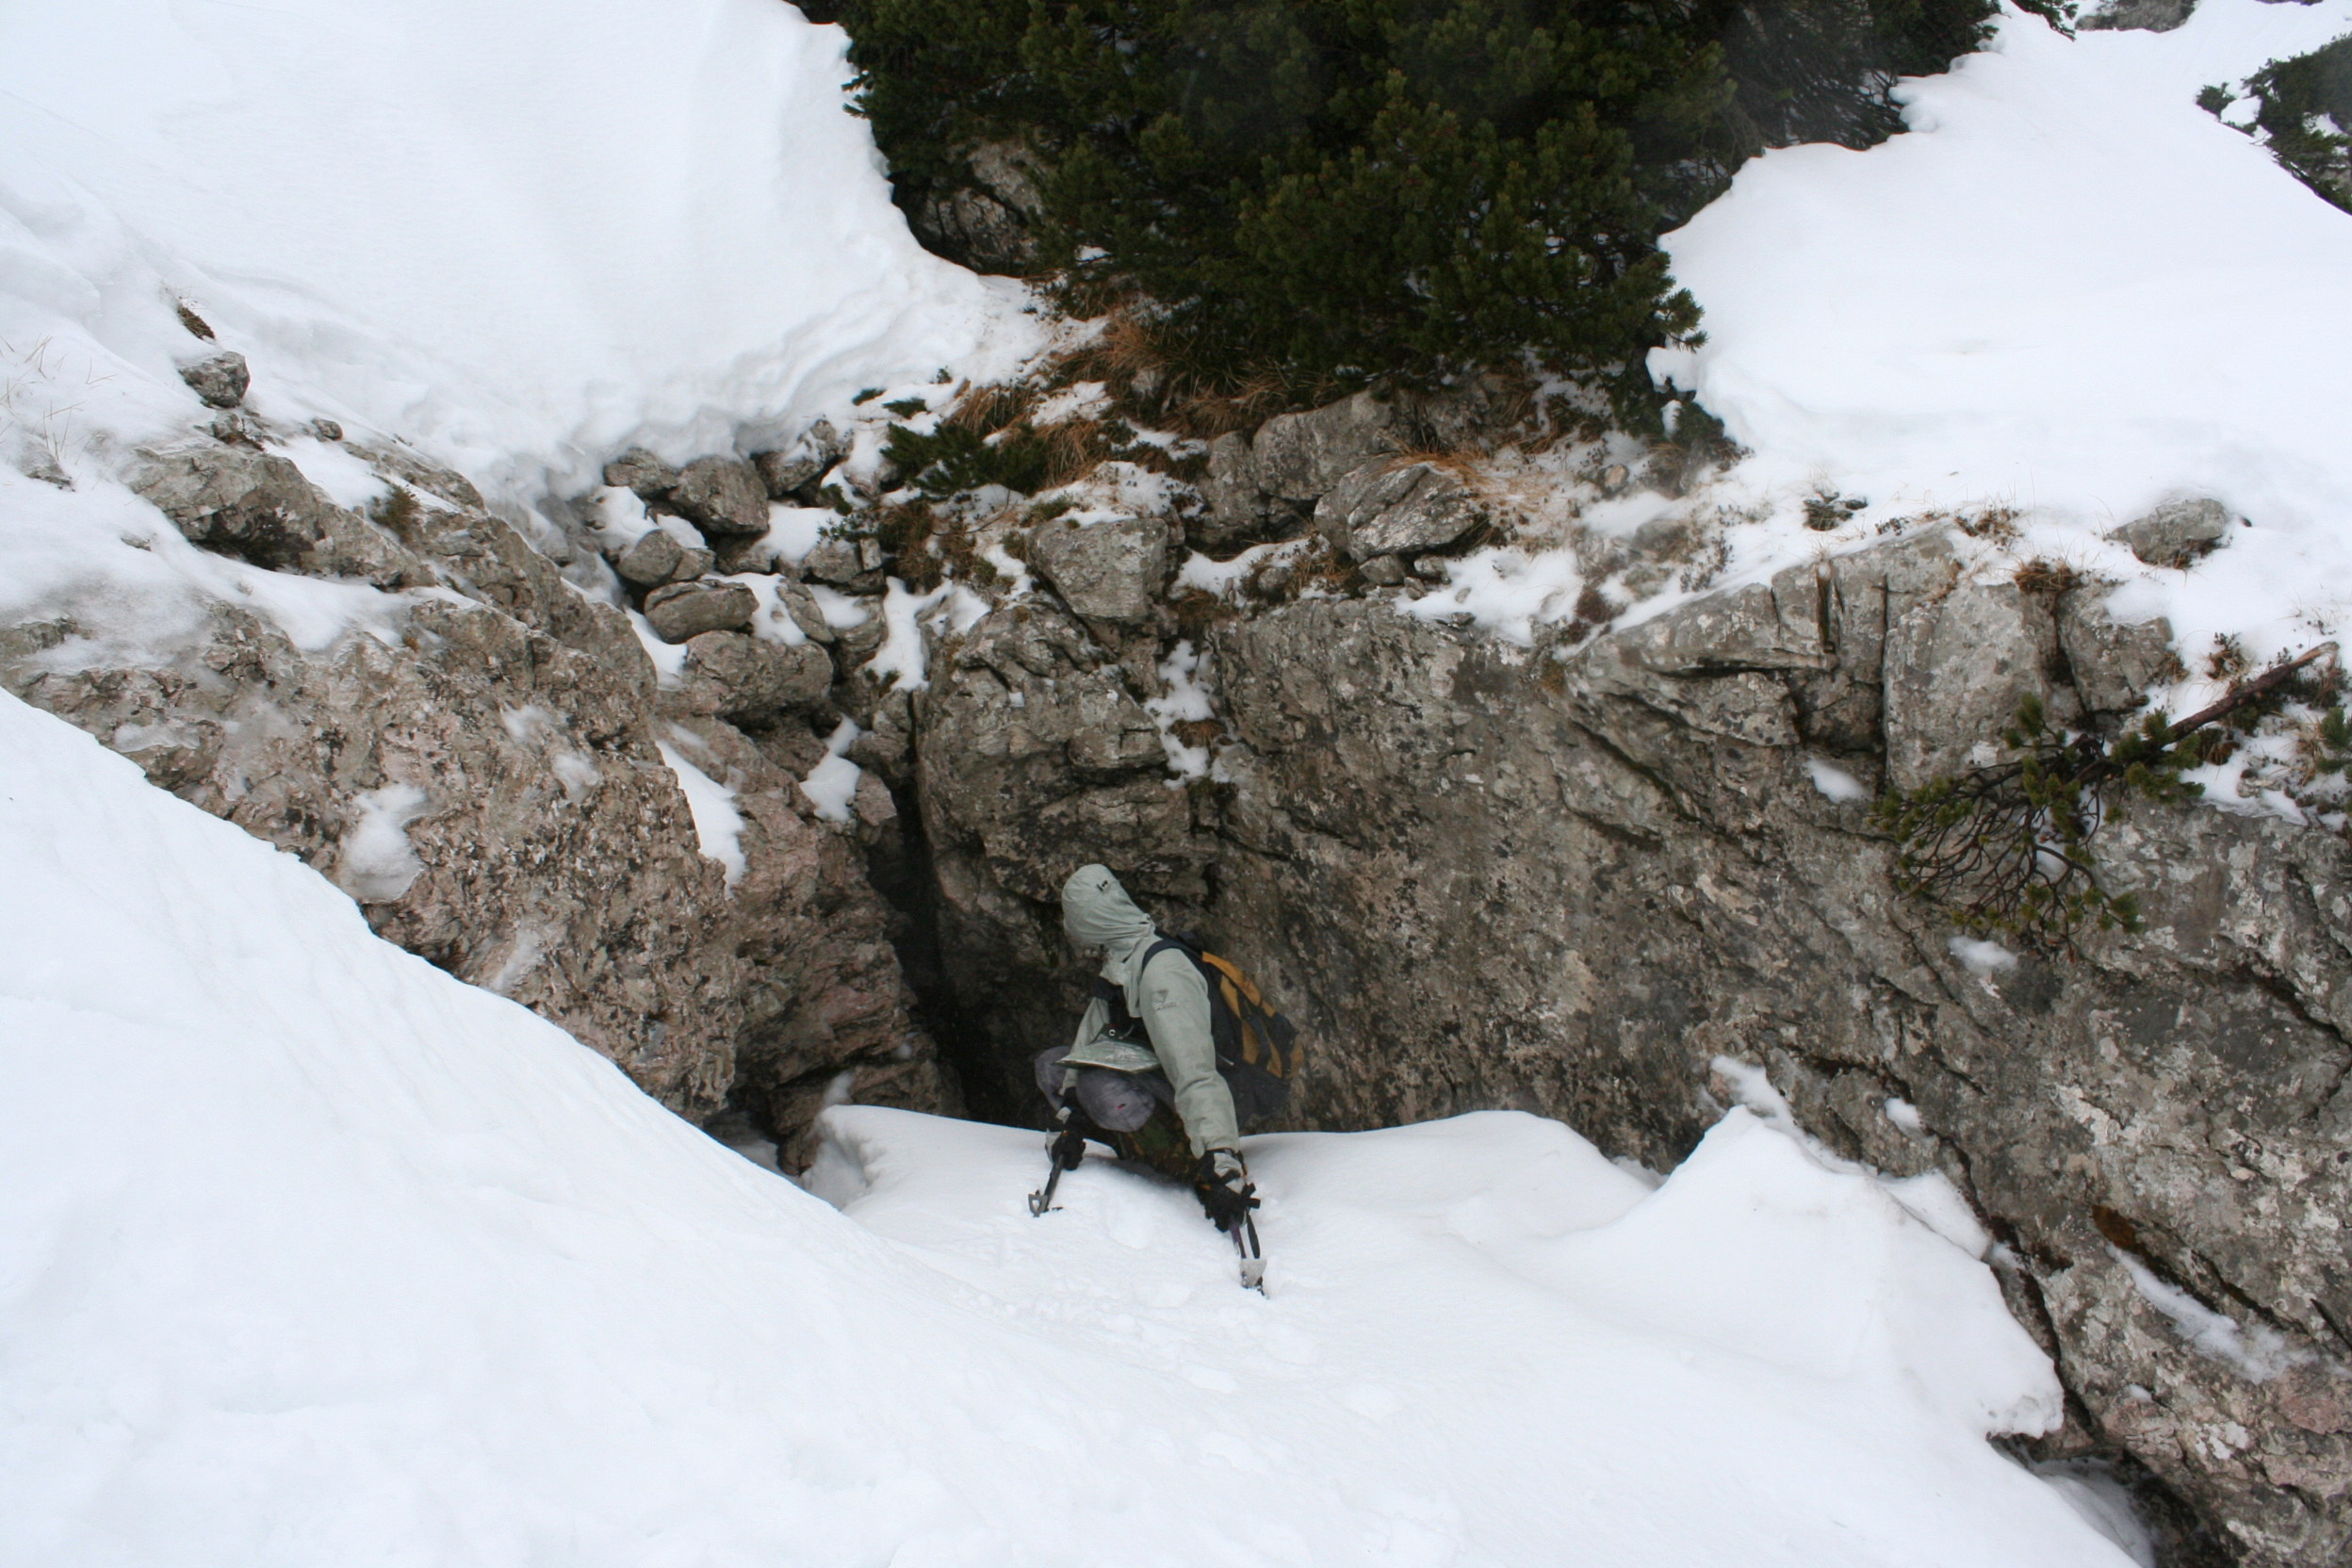
\includegraphics[width=\linewidth]{2009/winter_recce/2009-12-30 - Area N Winter Recce - Jana Carga - Canon 350d - IMG_7305-N6--orig.jpg}} 
        \caption{} \label{N6}
\end{subfigure}
\hfill
\begin{subfigure}{0.49\textwidth}
    \centering
        \frame{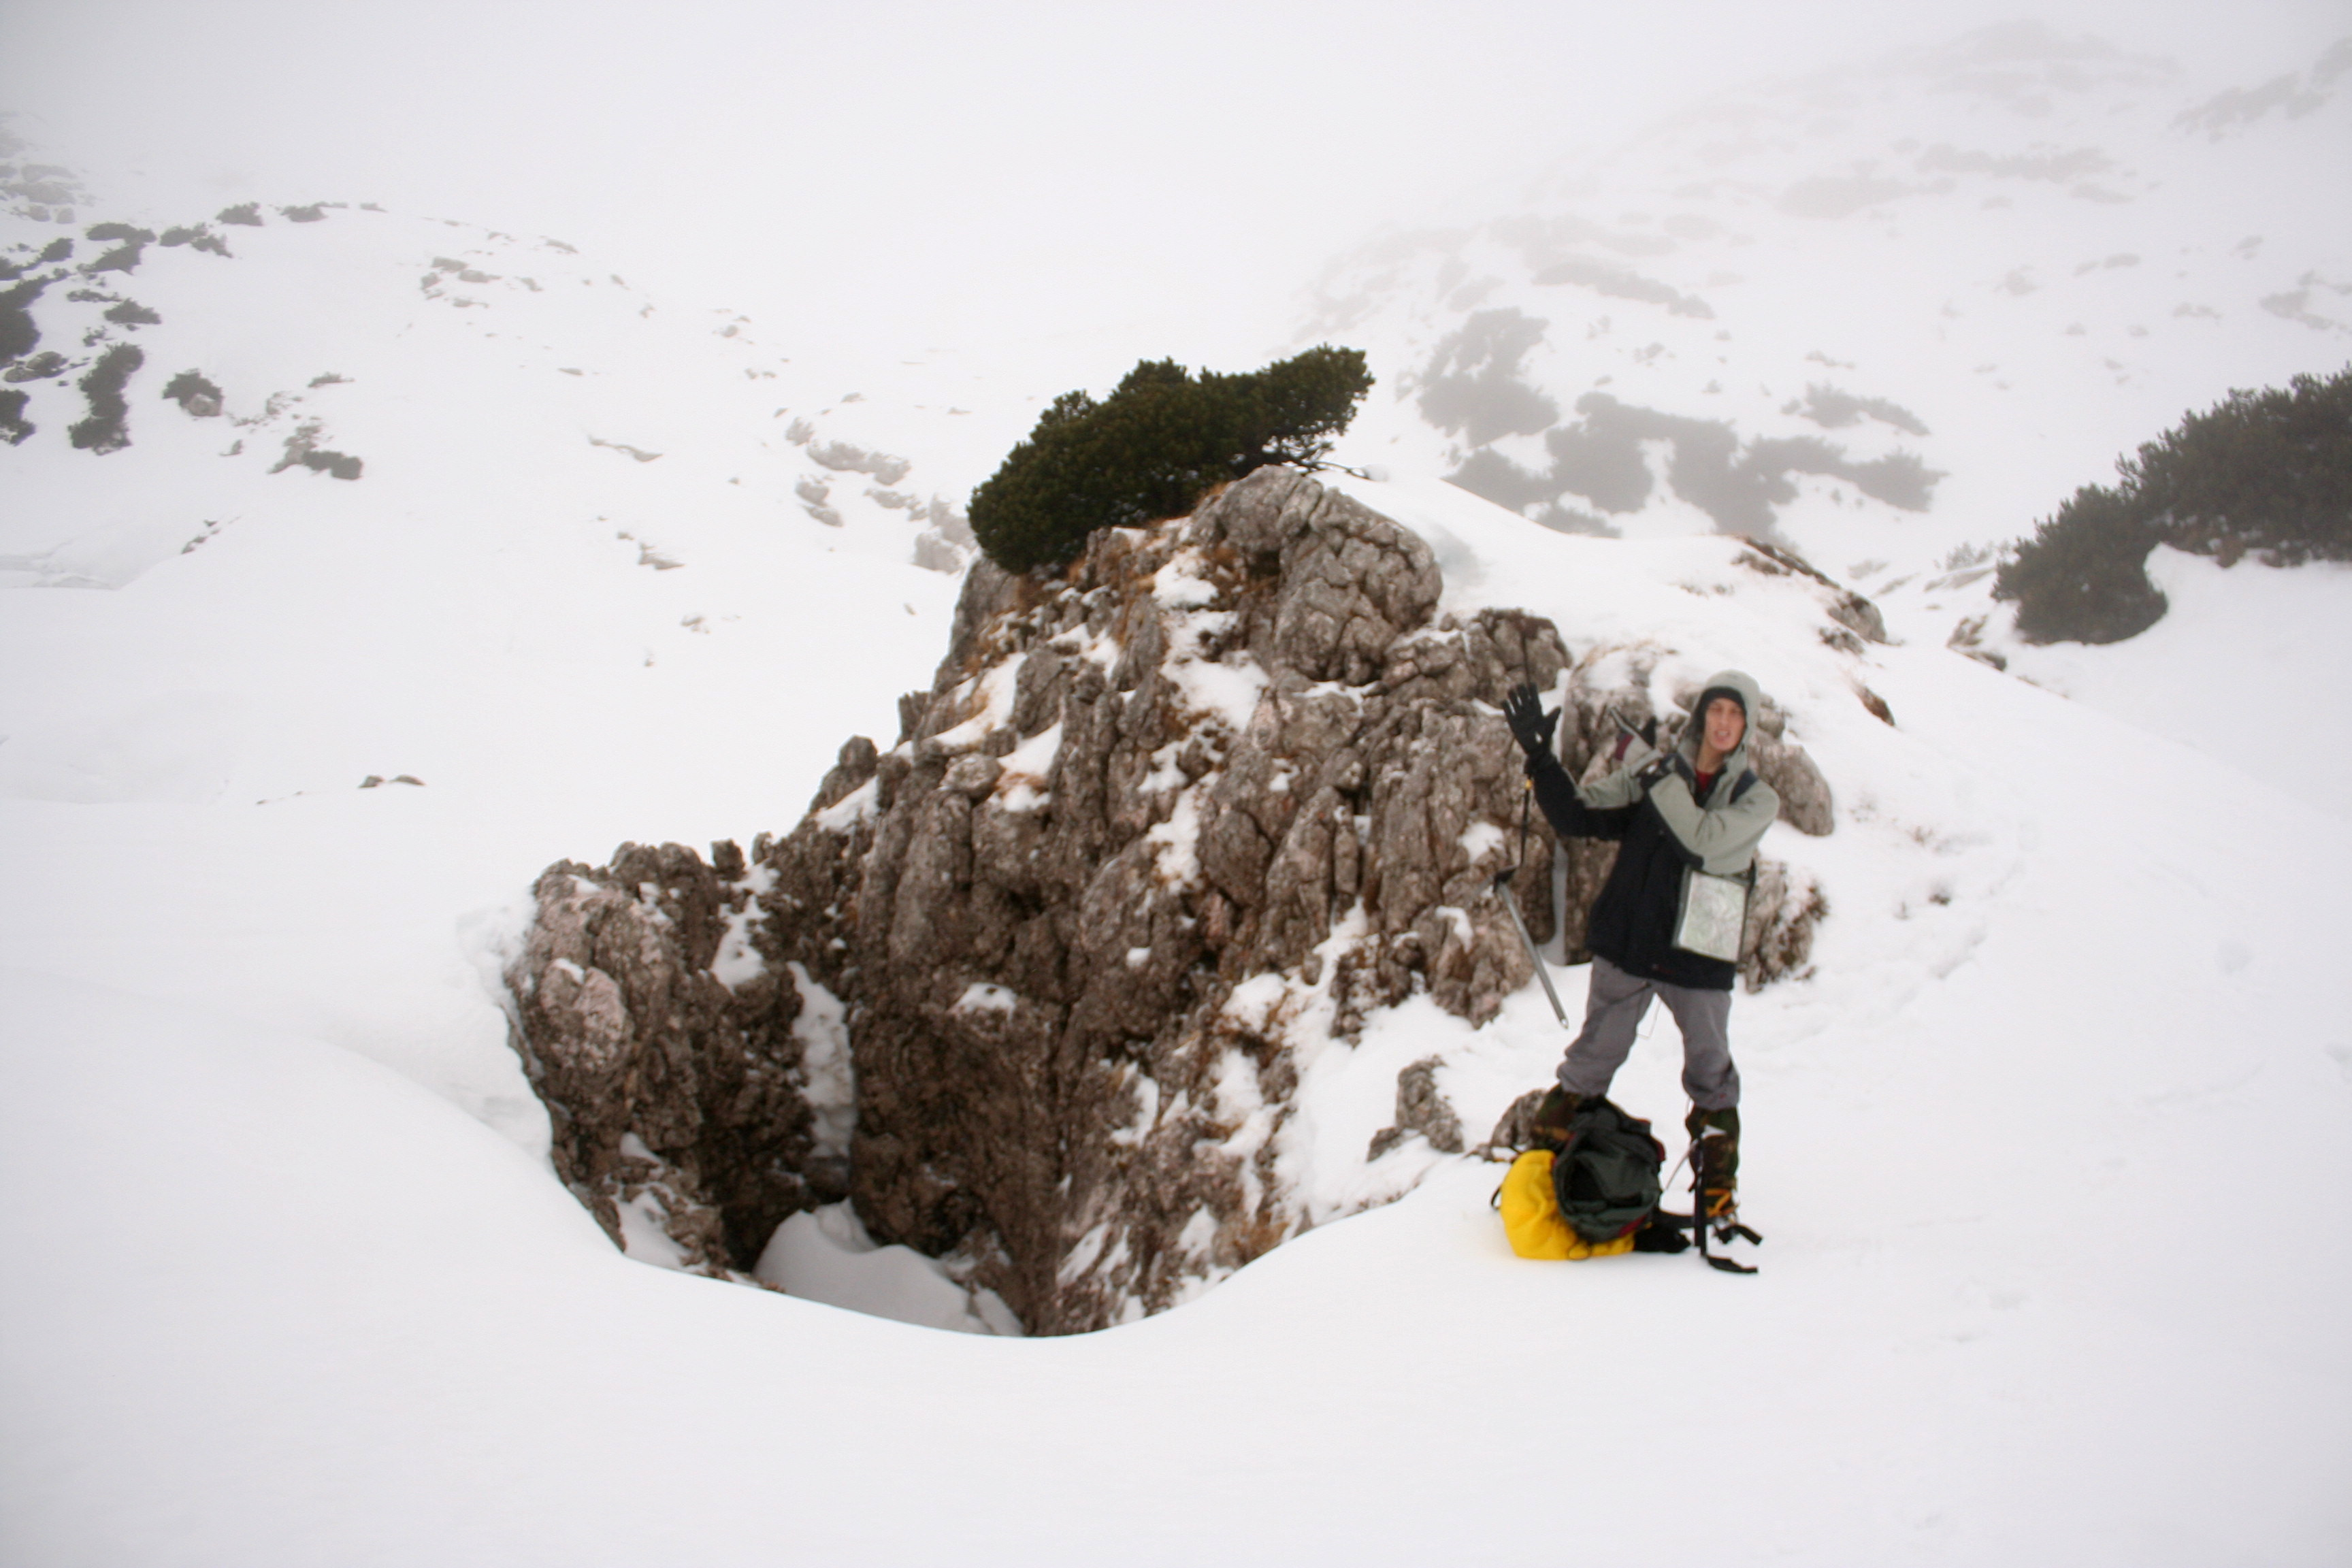
\includegraphics[width=\linewidth]{2009/winter_recce/2009-12-30 - Area N Winter Recce - Jana Carga - Canon 350d - IMG_7310-N7--orig.jpg}} 
        \caption{} \label{N7 1}
    \end{subfigure}
 \caption{\protect\passage{N3}, \protect\passage{N6}, \protect\passage{N7} and \protect\passage{N10}. \textit{(a)} The entrance of \protect\passage{N3}. \textit{(b)} Jarvist at the blowing hole \protect\passage{N10}, with N3 in the background. \textit{(c)} The entrance of \protect\passage{N6}. \textit{(d)} The entrance of \protect\passage{N7}. \pic{Jana Čarga} }
\end{pagefigure}







\begin{pagefigure}
      \checkoddpage \ifoddpage \forcerectofloat \else \forceversofloat \fi
    \centering
    \begin{subfigure}{0.49\textwidth}
        \frame{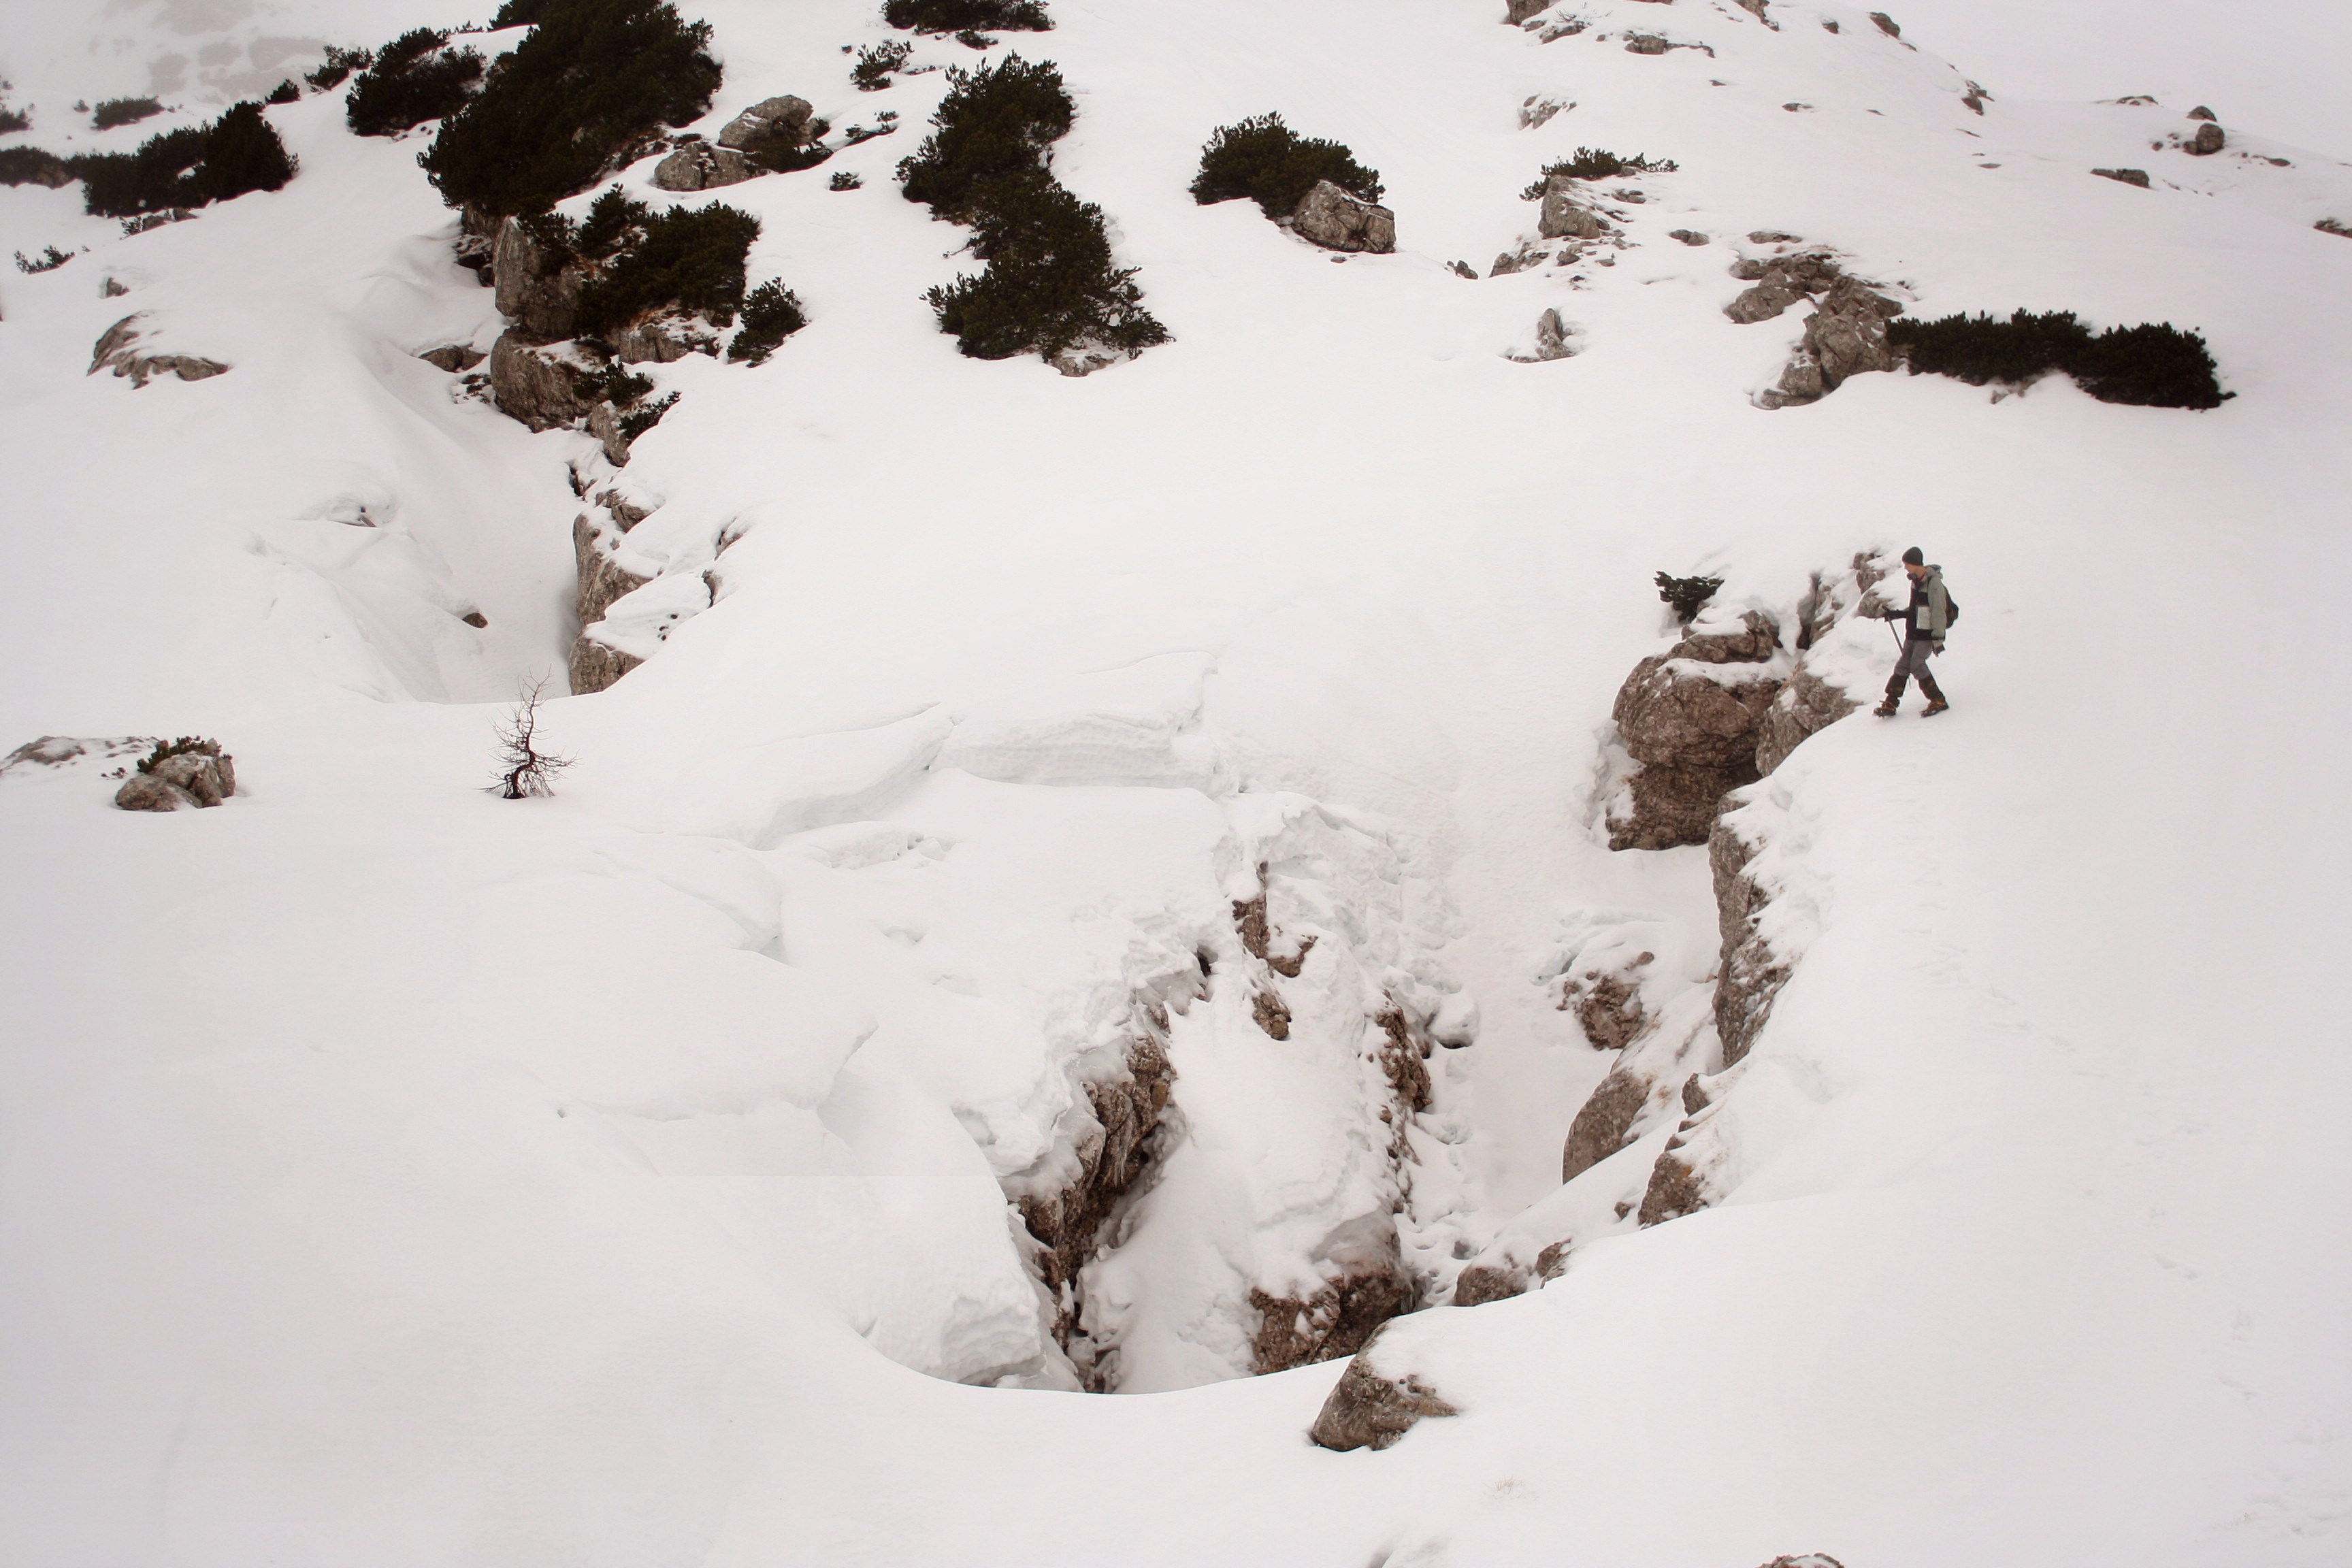
\includegraphics[width=\linewidth]{2009/winter_recce/2009-12-30 - Area N Winter Recce - Jana Carga - Canon 350d - IMG_7312-jarv approaching N8--orig.jpg}} 
        \caption{} \label{N8 1}
    \end{subfigure}
\hfill
    \begin{subfigure}{0.49\textwidth}
    \centering
        \frame{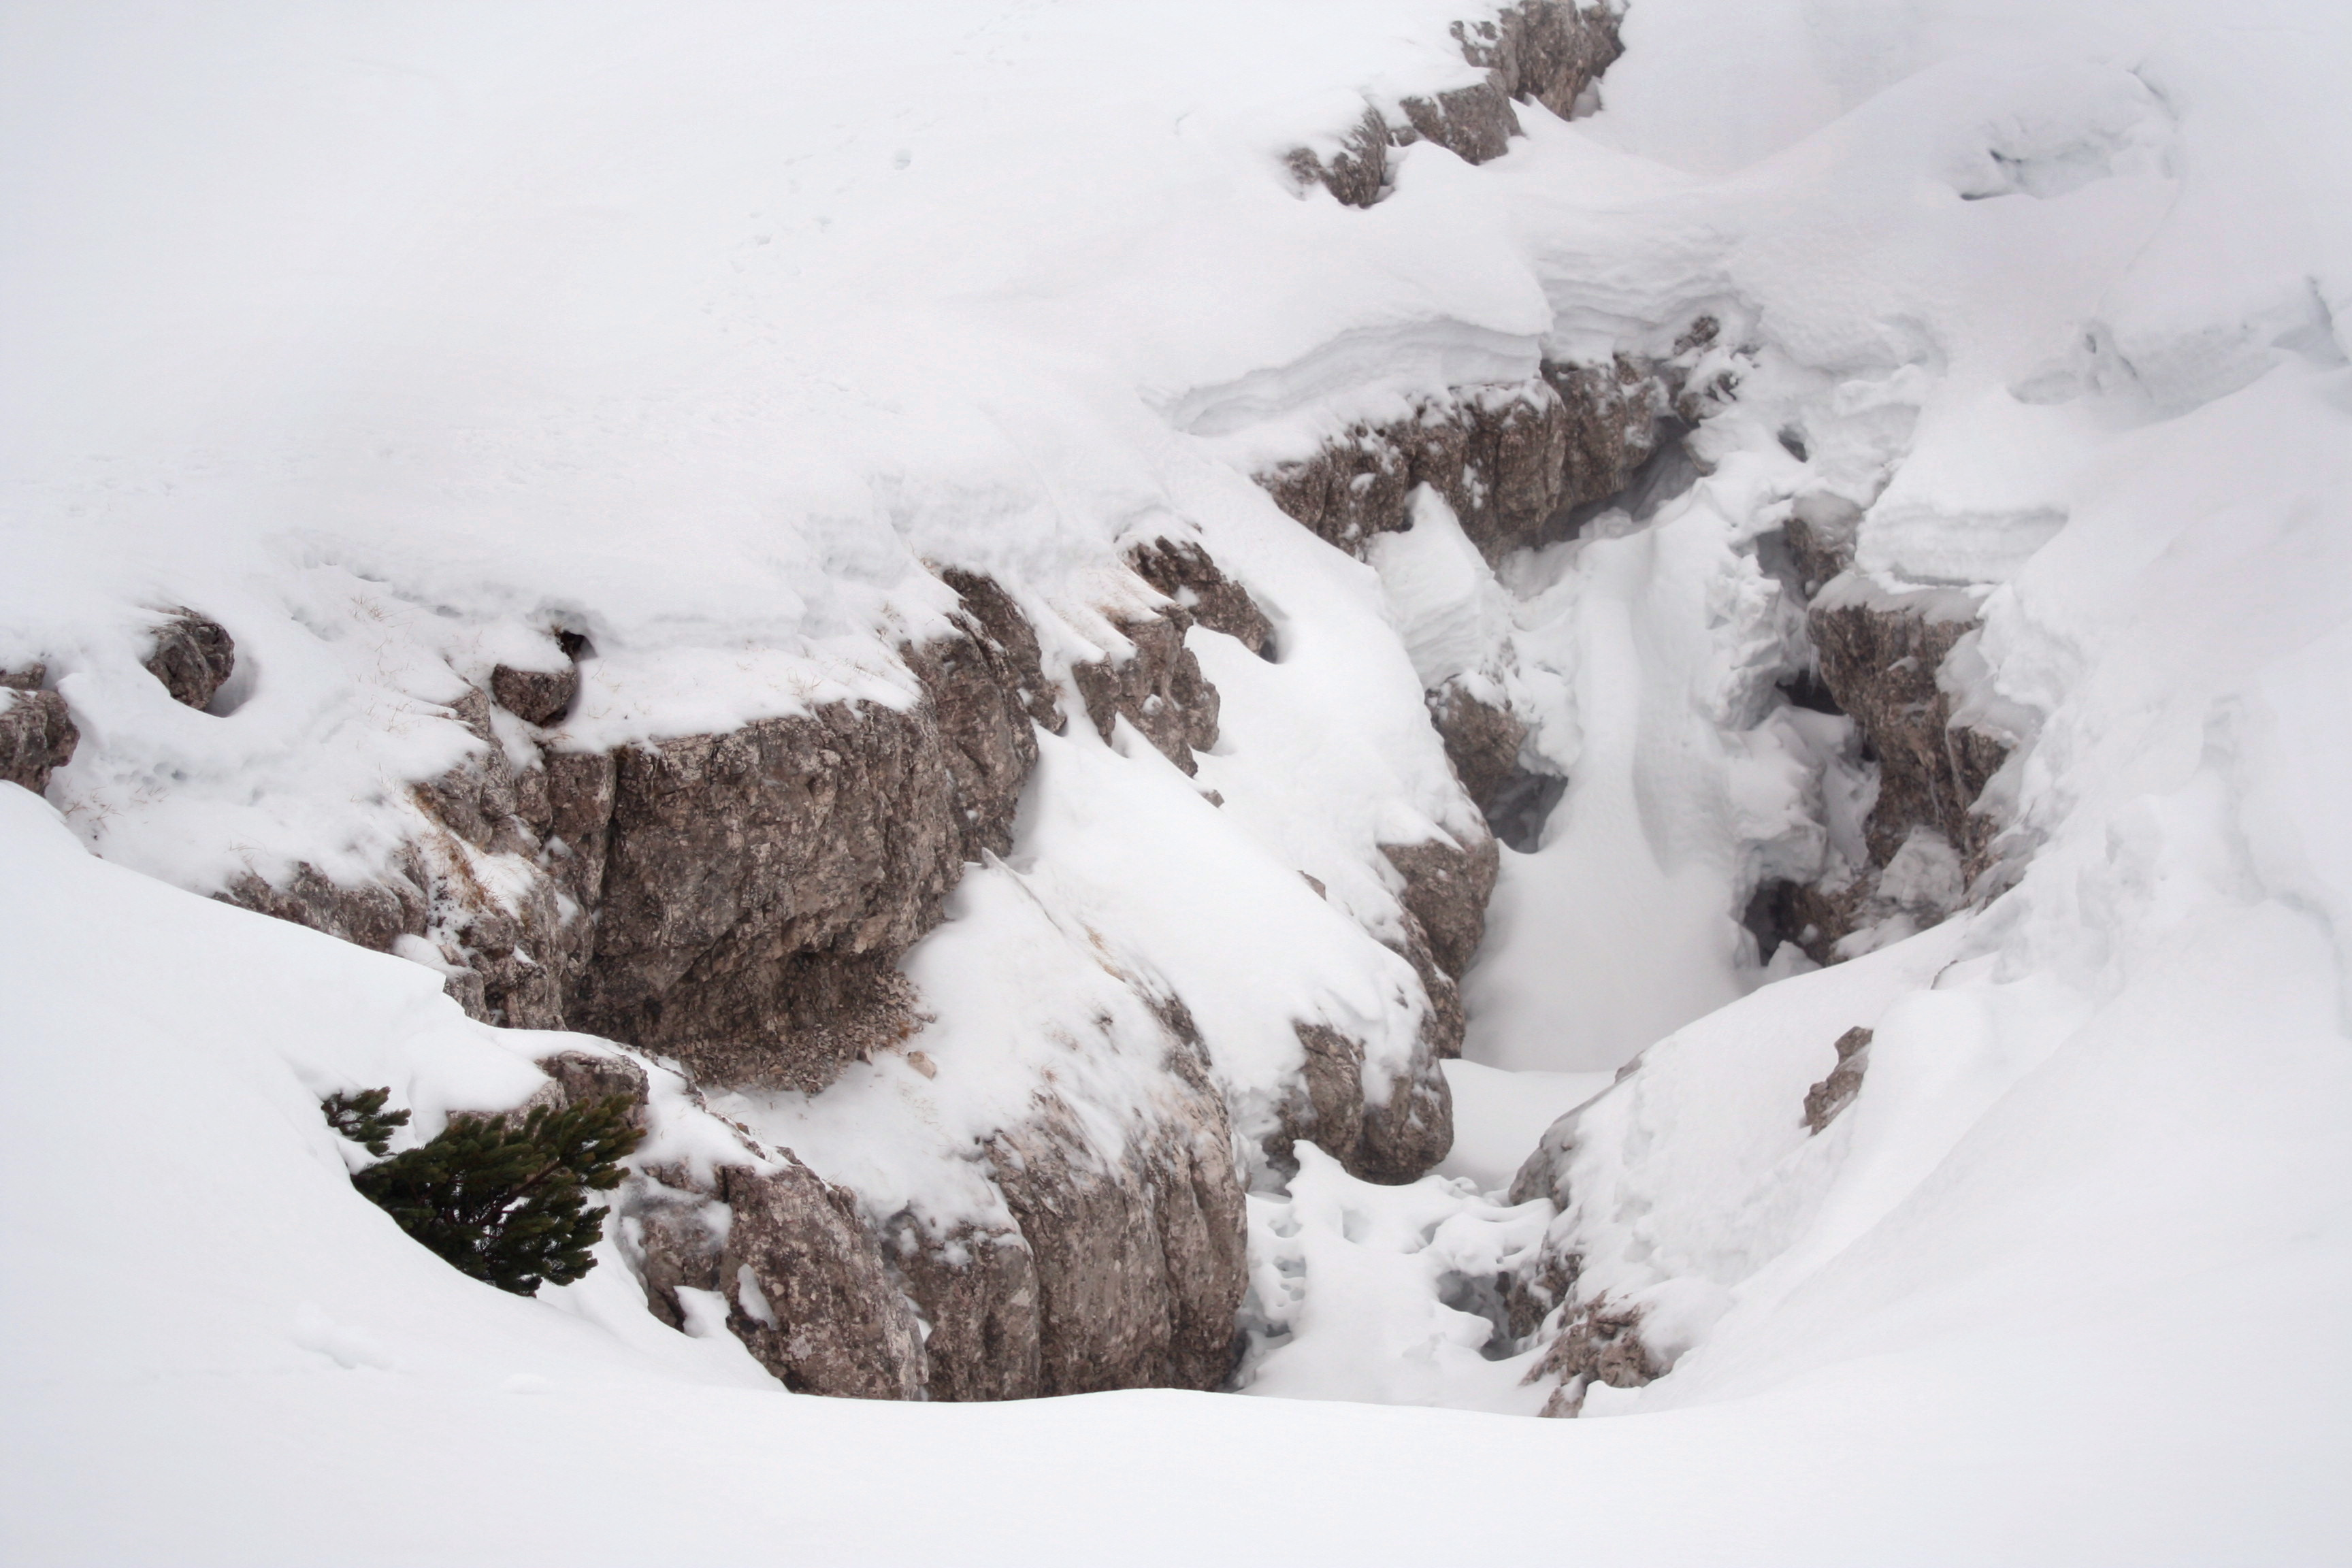
\includegraphics[width=\linewidth]{2009/winter_recce/2009-12-30 - Area N Winter Recce - Jana Carga - Canon 350d - IMG_7313-N8--orig.jpg}} 
        \caption{} \label{N8 2}
\end{subfigure}
\vfill
\begin{subfigure}{0.49\textwidth}
    \centering
        \frame{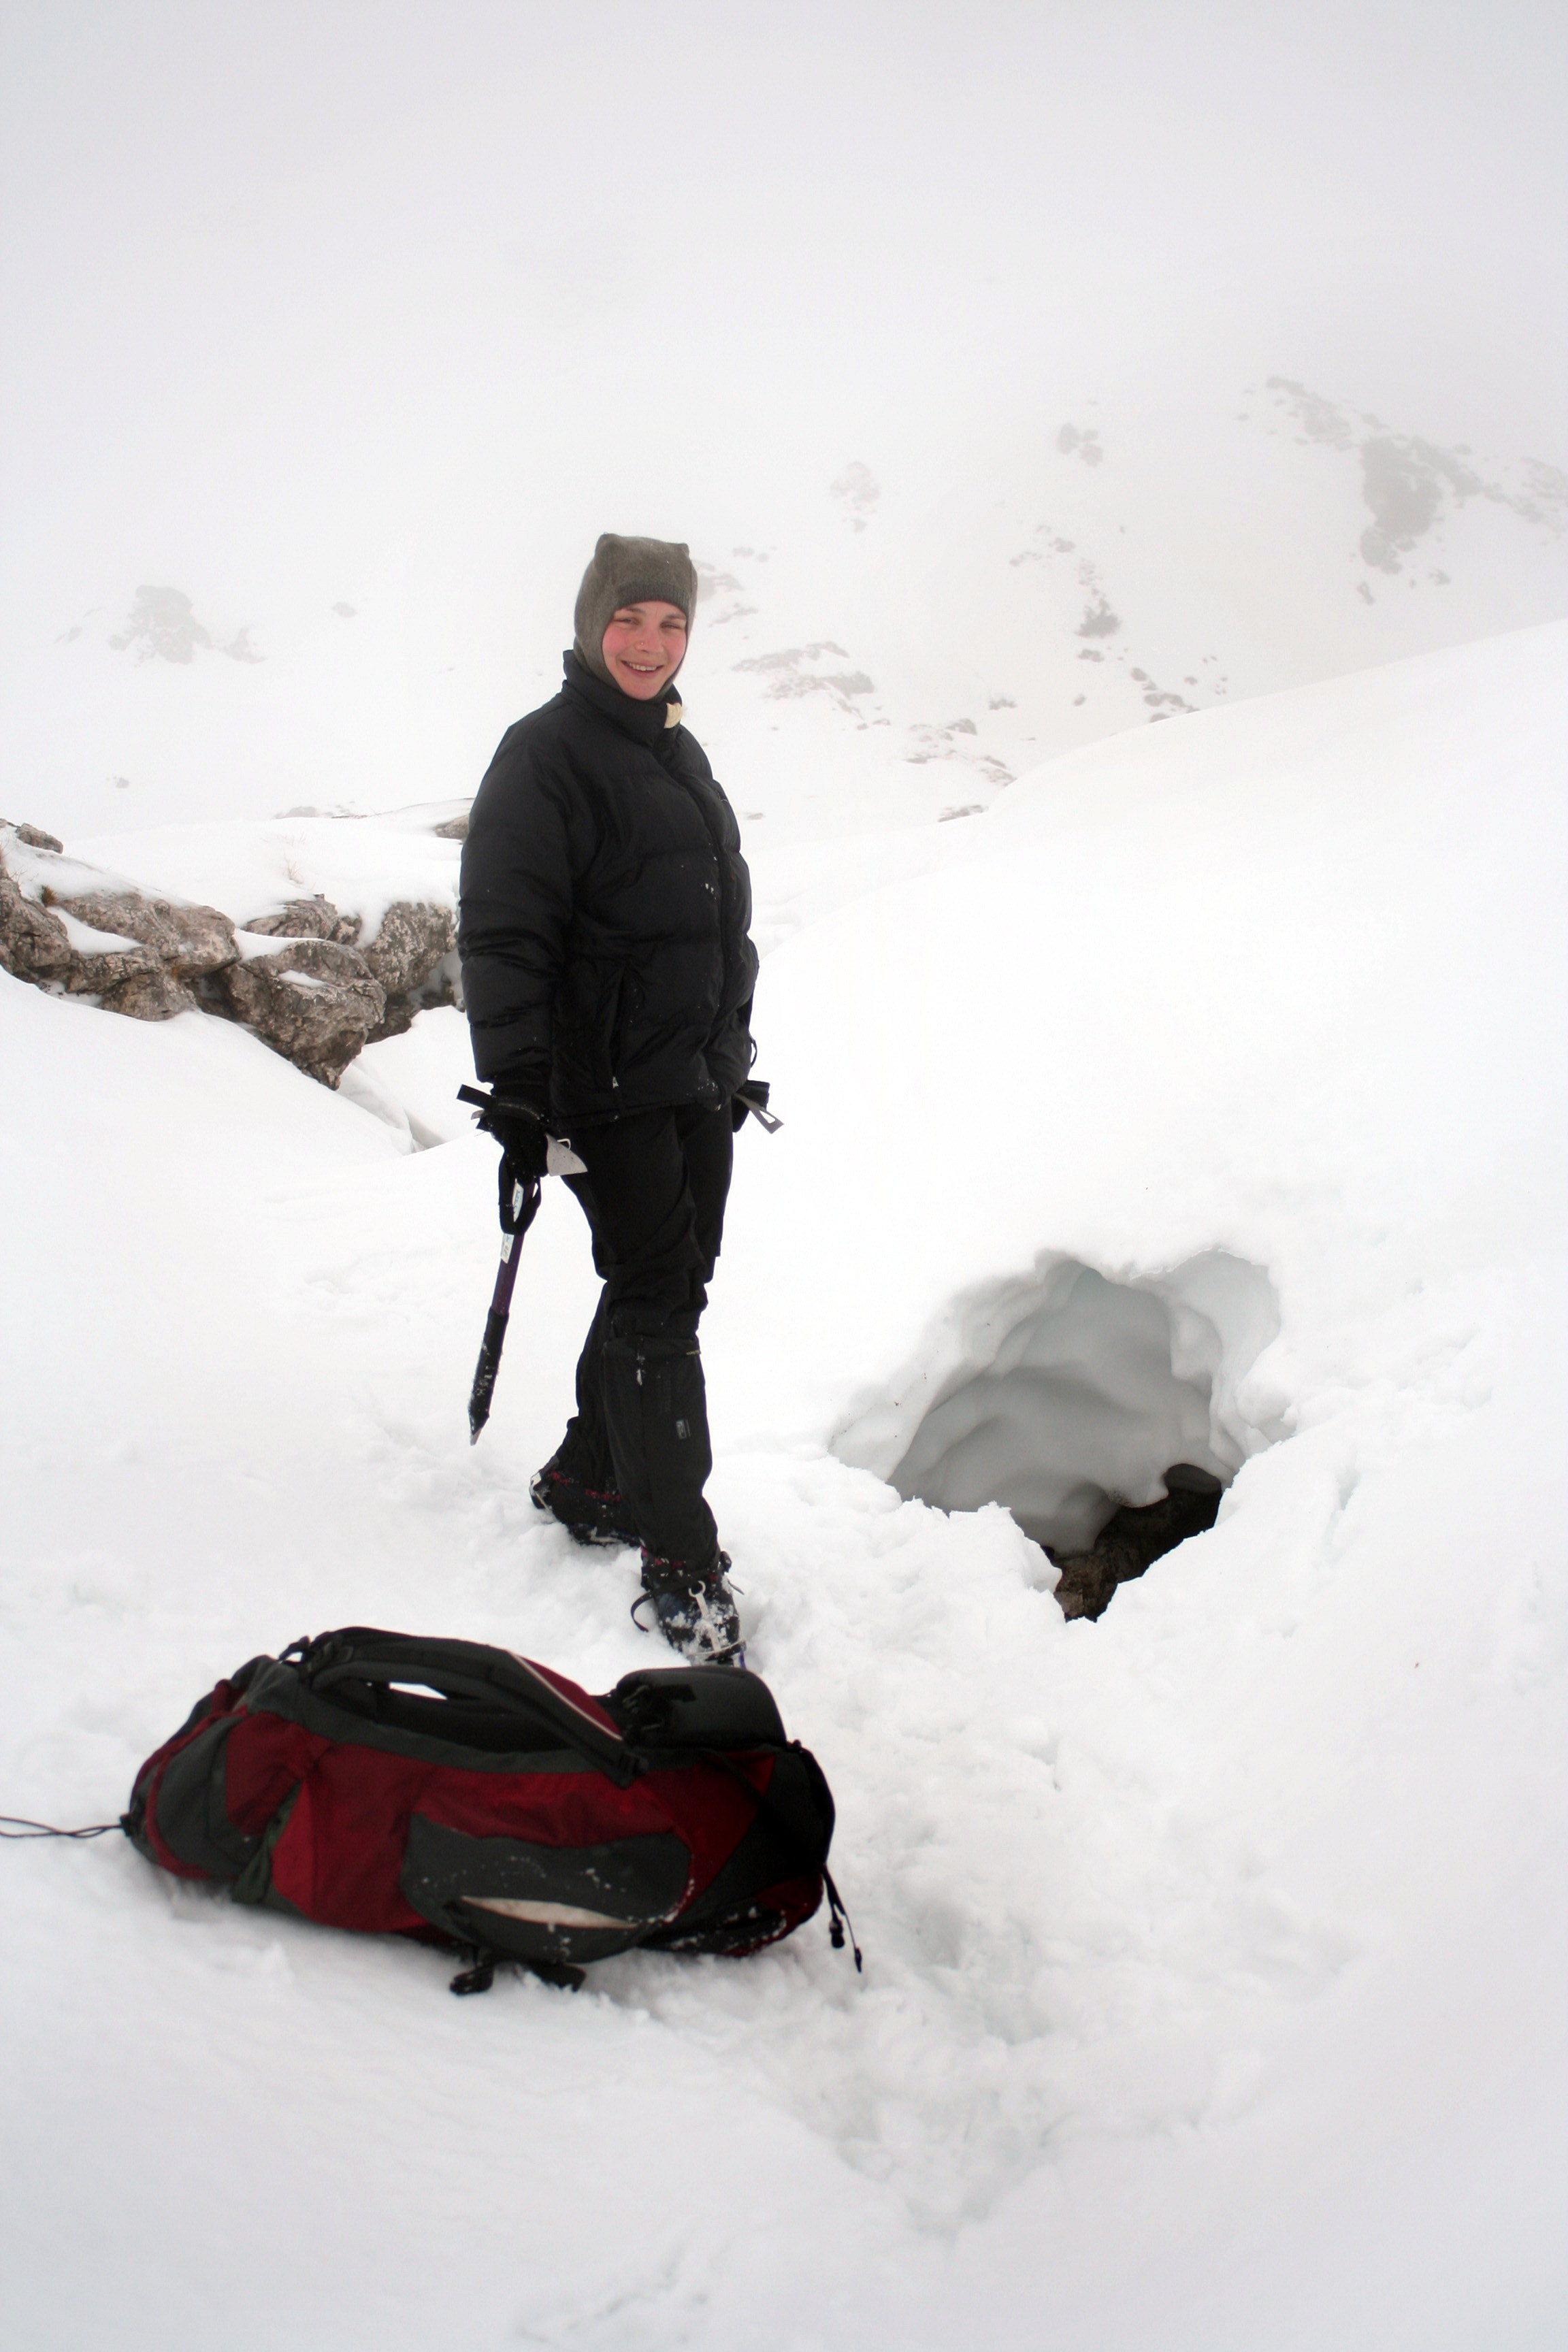
\includegraphics[width=\linewidth]{2009/winter_recce/2009-12-30 - Area N Winter Recce - Jana Carga - Canon 350d - IMG_7317-Jana posing next to N9--orig.jpg}} 
        \caption{} \label{N9 1}
\end{subfigure}
\hfill
\begin{subfigure}{0.49\textwidth}
    \centering
        \frame{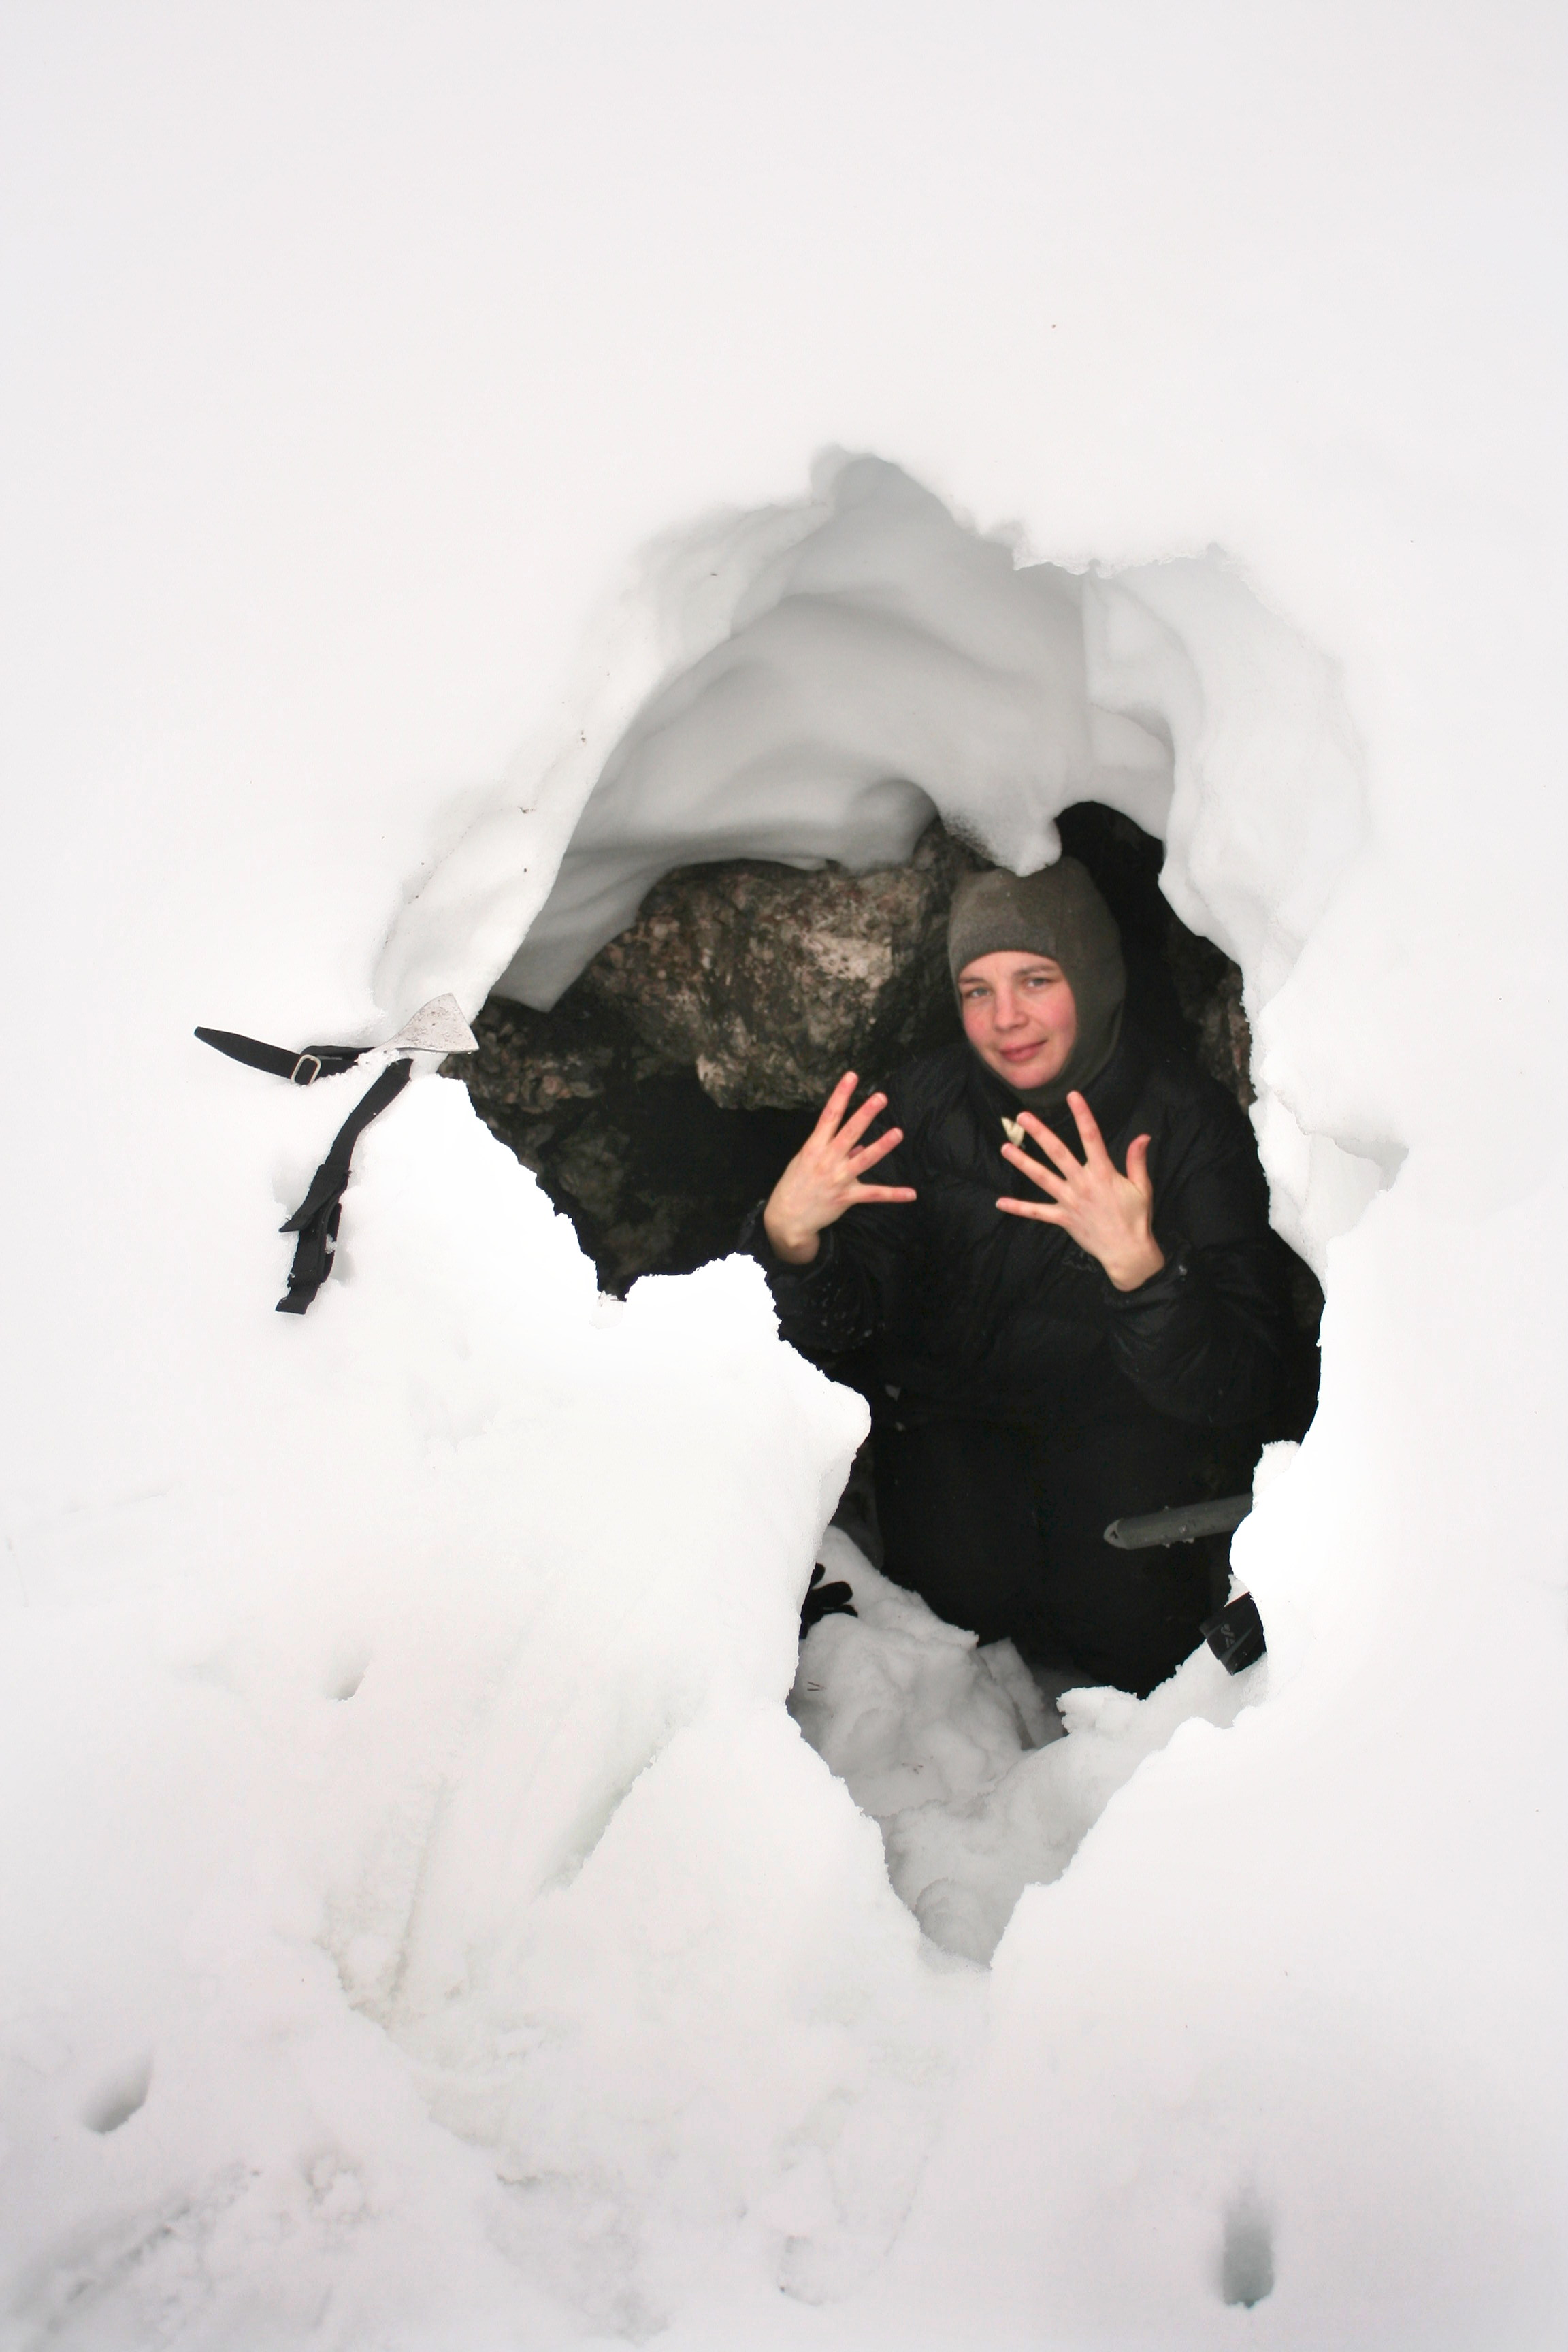
\includegraphics[width=\linewidth]{2009/winter_recce/2009-12-30 - Area N Winter Recce - Jana Carga - Canon 350d - IMG_7316-N9 Jana in entrance--orig.jpg}}
        \caption{} \label{N9 2}
    \end{subfigure}
 \caption{\protect\passage{N8} and \protect\passage{N9} (AKA \protect\passage{Kuk Pot}). \textit{(a)} Jarvist approaching \protect\passage{N8}. \textit{(b)} The shakehole of \protect\passage{N8}. \textit{(c)} Jana beside the blowing hole of \protect\passage{N9}. \textit{(d)} Jana in the entrance of \protect\passage{N9}. \pic{Jana Čarga / Jarvist Frost} }
\end{pagefigure}